% DM d'optimisation (CentraleSupélec) -- décodage spéculatif -- VERSION INTERMÉDIAIRE
% Compilation : pdflatex rapport_dm_intermediaire.tex (deux passes pour les références croisées)
\documentclass[11pt,a4paper]{article}
\usepackage[utf8]{inputenc}
\usepackage[T1]{fontenc}
\usepackage{lmodern}
\usepackage[french]{babel}
\frenchsetup{SmallCapsFigTabCaptions=false,og=«,fg=»}
\usepackage[a4paper,margin=2.2cm]{geometry}
\usepackage{amsmath,amssymb,amsthm,mathtools}
\usepackage{graphicx}
\usepackage{tikz}
\usetikzlibrary{positioning}
\usepackage{pifont}
\usepackage{booktabs,tabularx,array}
\usepackage{enumitem}
\usepackage{calc}
\usepackage[dvipsnames]{xcolor}
\usepackage{microtype}
\usepackage{caption}
\usepackage[colorlinks=true,linkcolor=MidnightBlue,citecolor=MidnightBlue,urlcolor=MidnightBlue]{hyperref}
\usepackage{xurl}

\captionsetup{font=small,labelfont=bf,format=hang,justification=justified}
\setlist{itemsep=2pt,topsep=3pt}
\setlength{\parskip}{3pt}
\graphicspath{{figures/}}

\newcommand{\R}{\mathbb{R}}
\newcommand{\TV}{\mathrm{TV}}
\newcommand{\Prob}{\mathbb{P}}
\newcommand{\Esp}{\mathbb{E}}
\newcommand{\sca}[2]{\langle #1,#2\rangle}
\newcommand{\nr}[1]{\|#1\|}
\newcommand{\clip}{\operatorname{clip}}
\newcommand{\vecop}{\operatorname{vec}}
\newcommand{\diag}{\operatorname{diag}}
\newcommand{\rg}{\operatorname{rg}}
\newcommand{\cB}{\mathcal{B}}
\newcommand{\cN}{\mathcal{N}}
\newcommand{\barre}[1]{\leavevmode\rlap{\rule[0.55ex]{\widthof{#1}}{0.5pt}}#1}
\newcommand{\tok}[1]{\texttt{#1}}

\theoremstyle{plain}
\newtheorem{proposition}{Proposition}
\newtheorem{lemme}{Lemme}
\theoremstyle{definition}
\newtheorem{exemple}{Exemple}
\newtheorem*{remarque}{Remarque}
\newtheorem*{suite}{Suite de l'exemple du §\ref{sec:regle}}

\title{\textbf{Où relâcher la vérification ?}\\[2pt]
\large Allocation optimale d'un budget de déviation en décodage spéculatif}
\author{Omar~Besbes \and Houssem~Guermazi\\[2pt]
\small DM d'optimisation, CentraleSupélec, dominante Mathématiques et Sciences des Données, 2026--2027}
\date{}

\begin{document}
\maketitle

\begin{abstract}
Les grands modèles de langage (LLM), qui animent les assistants conversationnels, écrivent un texte morceau de mot par morceau de mot, et chaque morceau coûte un calcul complet du modèle : la génération est lente.
Le \emph{décodage spéculatif} l'accélère : un petit modèle rapide (le \emph{draft}) propose plusieurs morceaux d'avance, et le grand modèle (le \emph{target}) les vérifie tous en un seul calcul.
Ce DM, issu de notre projet de recherche en apprentissage automatique, étudie deux problèmes d'optimisation posés par cette vérification.
\textbf{(I)} Vérifier un morceau proposé est un programme linéaire de transport : notre simplexe et un certificat dual montrent que la probabilité d'acceptation maximale vaut $1-\TV(p,q)$, et qu'une petite déviation $\varepsilon$ tolérée sur le texte produit la porte à $\min(1,1-\TV+\varepsilon)$.
\textbf{(II)} Répartir un budget de déviation entre les positions d'un bloc proposé est un problème \emph{non concave} sous contraintes linéaires, que nous traitons par les conditions KKT et le gradient projeté.
Comme un rejet interrompt le bloc, il faut dévier d'abord sur les \textbf{premières} positions : dans un scénario typique, on va ainsi 26\,\% plus vite qu'avec une règle qui ignore cette structure.
\end{abstract}

\begin{center}
\small
\begin{tabularx}{\linewidth}{@{}>{\raggedright}p{0.36\linewidth}X@{}}
\toprule
\textbf{Attendu du DM} & \textbf{Où} \\\midrule
Modélisation & §\ref{sec:modeleI} (PL), §\ref{sec:modeleII} (allocation)\\
Existence et unicité & §\ref{sec:existenceI} (PL : non-unicité caractérisée), §\ref{sec:existenceII} (non-concavité, cas $\gamma=2$)\\
Théorèmes du cours~\cite{allaire}, conditions d'optimalité & dualité en PL (§\ref{sec:dualite}), conditions de Karush-Kuhn-Tucker (§\ref{sec:kkt}), inéquation d'Euler (annexe~\ref{app:convergence})\\
Algorithme et convergence & simplexe en deux phases (§\ref{sec:simplexe}), gradient projeté (§\ref{sec:algoII}, annexe~\ref{app:convergence})\\
Plusieurs minima locaux ? & objectif non concave, multi-départs (§\ref{sec:algoII})\\
Originalité & \textbf{méthode du simplexe}, \textbf{mise en œuvre de la dualité} (certificat, prix duaux)\\
\bottomrule
\end{tabularx}
\end{center}

%=====================================================================
\section{Introduction : accélérer un modèle de langage}\label{sec:contexte}
%=====================================================================
\subsection{Un modèle de langage, vu par un optimiseur}\label{sec:llm}
Un texte est découpé en \textbf{tokens} : des mots ou des morceaux de mots, pris dans un vocabulaire fixe de $n$ éléments ($n\approx150\,000$ pour les modèles utilisés ici).
Un \textbf{modèle de langage} est une fonction qui associe au début d'un texte une loi de probabilité $p\in\Delta_n=\{p\in\R_+^n:\sum_ip_i=1\}$ sur le token suivant.
Par exemple (valeurs illustratives), après « Le chat dort sur le », un modèle pourrait donner :
\begin{center}\small
\begin{tabular}{@{}lccccc@{}}
\toprule
token suivant & \tok{canapé} & \tok{lit} & \tok{tapis} & \tok{toit} & autres\\
probabilité & 0,40 & 0,25 & 0,20 & 0,05 & 0,10\\
\bottomrule
\end{tabular}
\end{center}
Pour écrire, on tire un token selon $p$, on l'ajoute au texte et l'on recommence : c'est la génération \textbf{autorégressive}.
Chaque token demande une \textbf{passe} du modèle, c'est-à-dire un calcul complet d'un réseau de neurones qui compte des milliards de paramètres, et ces passes sont séquentielles, puisque chaque token dépend des précédents.
Une réponse de 500 tokens coûte 500 passes successives : c'est le goulot d'étranglement.
Un fait technique permet d'aller plus vite : en \emph{une} passe, le modèle calcule la loi du token suivant à \emph{toutes} les positions d'un texte donné (c'est ainsi qu'il est entraîné). Vérifier $\gamma$ tokens déjà écrits coûte donc à peu près autant que d'en générer un seul.

\subsection{Le décodage spéculatif : un petit modèle propose, le grand vérifie}\label{sec:specdec}
On dispose de deux modèles : le \textbf{target}, grand et lent, dont on veut la qualité (ici Qwen2.5-1.5B, de loi $p$), et le \textbf{draft}, petit et rapide (Qwen2.5-0.5B, de loi $q$).
À chaque étape, le draft propose un \textbf{bloc} de $\gamma$ tokens, l'un après l'autre, ce qui est peu coûteux.
Le target les examine tous en une seule passe et les accepte de gauche à droite tant qu'ils passent la vérification.
Au premier rejet, il remplace le token rejeté par le sien et jette la fin du bloc ; si tout est accepté, il ajoute un token de plus.
Une passe du target produit donc entre 1 et $\gamma+1$ tokens au lieu d'un seul (figure~\ref{fig:specdec}), et la \textbf{vitesse} se mesure par le nombre moyen de tokens produits par passe du target.
Sur les solutions de deux problèmes de mathématiques du jeu de données GSM8K, le target produit ainsi en moyenne 4,76 et 4,59 tokens par passe.

\begin{figure}[htbp]
\centering
\begin{tikzpicture}[
  tok/.style={draw, rounded corners=2pt, minimum height=6.5mm, inner xsep=4pt, font=\ttfamily\small},
  acc/.style={tok, fill=ForestGreen!12, draw=ForestGreen!80!black},
  rej/.style={tok, fill=red!10, draw=red!75!black},
  tgt/.style={tok, fill=MidnightBlue!12, draw=MidnightBlue},
  jet/.style={tok, fill=gray!8, draw=gray!50, text=gray},
  titre/.style={font=\small\bfseries, anchor=west},
  expl/.style={font=\small, align=left, anchor=west},
  node distance=1.6mm]
\node[titre] at (-0.1,1.1) {Passe 1 : tout le bloc est accepté};
\node[acc, anchor=west] (a1) at (0,0) {out};
\node[acc, right=of a1] (a2) {how};
\node[acc, right=of a2] (a3) {many};
\node[acc, right=of a3] (a4) {miles};
\node[acc, right=of a4] (a5) {Brian};
\node[tgt, right=3mm of a5] (a6) {+1};
\foreach \i in {1,...,5} \node[font=\small, text=ForestGreen!80!black, above=0.2mm of a\i] {\ding{51}};
\node[expl] at (8.0,0) {5 tokens acceptés + 1 token du target\\$=$ \textbf{6 tokens} pour une passe};
\node[titre] at (-0.1,-0.9) {Passe 2 : rejet en position 3};
\node[acc, anchor=west] (b1) at (0,-2) {the};
\node[acc, right=of b1] (b2) {distance};
\node[rej, right=of b2] (b3) {Brian};
\node[jet, right=of b3] (b4) {\dots};
\node[jet, right=of b4] (b5) {\dots};
\foreach \i in {1,2} \node[font=\small, text=ForestGreen!80!black, above=0.2mm of b\i] {\ding{51}};
\node[font=\small, text=red!75!black, above=0.2mm of b3] {\ding{55}};
\node[font=\scriptsize, text=gray, above=0.4mm of b4.north east] {jetés};
\node[tgt, below=4mm of b3] (b3t) {Sof};
\draw[->, MidnightBlue] (b3.south) -- (b3t.north);
\node[font=\scriptsize, text=MidnightBlue, right=1mm of b3t] {choix du target};
\node[expl] at (8.0,-2) {2 tokens acceptés + 1 correction du target\\$=$ \textbf{3 tokens} pour une passe};
\end{tikzpicture}
\caption{Deux passes réelles sur un problème GSM8K (« Sofie marche deux fois plus que Brian\dots »), avec Qwen2.5-0.5B comme draft et Qwen2.5-1.5B comme target. Le draft propose 5 tokens ; le target les vérifie en une passe, en acceptant chaque token qui coïncide avec son propre choix (vert). Au premier désaccord (rouge), il émet son token (bleu) et jette la fin du bloc (gris). Sans draft, chaque passe ne produirait qu'un token.}
\label{fig:specdec}
\end{figure}

\subsection{Une règle de vérification qui ne change pas le texte produit}\label{sec:regle}
La figure~\ref{fig:specdec} utilise la vérification la plus simple : le target accepte un token s'il coïncide avec son choix le plus probable.
Pour échantillonner, c'est-à-dire tirer chaque token au hasard selon $p$ (ce qui donne des textes variés), la règle de Leviathan et al.~\cite{leviathan}, proposée indépendamment par Chen et al.~\cite{chen}, accepte le token $x$ proposé par le draft avec probabilité $\min(1,p_x/q_x)$ ; en cas de rejet, le target tire son token selon $(p-q)_+$ renormalisé.
Le texte produit suit alors \emph{exactement} la loi $p$ du target : on va plus vite sans rien changer à la qualité.

Prenons un vocabulaire de trois tokens (\tok{canapé}, \tok{lit}, \tok{tapis}), avec $p=(0{,}5;0{,}3;0{,}2)$ pour le target et $q=(0{,}2;0{,}3;0{,}5)$ pour le draft.
\begin{itemize}
\item Si le draft propose \tok{canapé} (probabilité 0,2) ou \tok{lit} (0,3), le target les veut au moins aussi souvent ($p_x\ge q_x$) : il accepte toujours.
\item Si le draft propose \tok{tapis} (probabilité 0,5), que le target ne veut qu'avec probabilité 0,2, il l'accepte avec probabilité $0{,}2/0{,}5=0{,}4$. Sinon (probabilité $0{,}5\times0{,}6=0{,}3$), il émet \tok{canapé}, le seul token que le draft propose moins souvent que lui.
\end{itemize}
Le texte produit contient \tok{canapé} avec probabilité $0{,}2+0{,}3=0{,}5$, \tok{lit} avec probabilité $0{,}3$ et \tok{tapis} avec probabilité $0{,}5\times0{,}4=0{,}2$ : c'est bien $p$.
Le token proposé est accepté avec probabilité $0{,}2+0{,}3+0{,}2=0{,}7=\sum_x\min(p_x,q_x)$.
\textbf{Peut-on accepter plus souvent, tout en produisant exactement $p$ ?} C'est la partie I : la réponse est non, et la question est un programme linéaire.

\subsection{Relâcher la vérification, mais où ?}\label{sec:ou}
Si l'on tolère que le texte produit s'écarte un peu de $p$, on peut accepter plus souvent : dans l'exemple, accepter toujours \tok{tapis} porte l'acceptation à 1, mais le texte suit alors la loi $q$ du petit modèle.
Entre les deux, une \textbf{déviation} $\varepsilon$ (l'écart permis entre la loi du texte produit et $p$, mesuré en variation totale) donne une acceptation $\min(1,0{,}7+\varepsilon)$ (proposition~\ref{prop:perte}).
Cette vérification \emph{avec perte}~\cite{fuzzy} soulève deux questions.

\textbf{Toutes les positions ne se valent pas pour la qualité.}
Sur GSM8K, la plupart des rejets portent sur des \textbf{synonymes} sans effet sur la réponse (\tok{determine} contre \tok{find}).
Quelques-uns portent sur des \textbf{pivots} qui orientent le raisonnement : dans la figure~\ref{fig:specdec}, le draft parle de la distance de Brian là où le target parle de celle de Sofie, et la suite du calcul en dépend ; ailleurs, il écrit « is \tok{not} » au lieu de « is \tok{left} », c'est-à-dire ce qui est utilisé au lieu de ce qui reste.
Dévier sur un synonyme ne coûte rien, mais dévier sur un pivot fausse la réponse : on attribue à chaque position une \textbf{sensibilité} $s_t$, le coût en qualité d'une unité de déviation.

\textbf{Toutes les positions ne se valent pas pour la vitesse.}
Un rejet interrompt le bloc : les premières positions conditionnent l'accès aux suivantes.
Avec $\gamma=3$ et des probabilités d'acceptation $(0{,}9;0{,}5;0{,}8)$, une passe produit en moyenne $1+0{,}9+0{,}9\times0{,}5+0{,}9\times0{,}5\times0{,}8=2{,}71$ tokens (formule du §\ref{sec:modeleII}) : la position 3, pourtant facile, n'est atteinte qu'une fois sur deux.
Gagner $0{,}1$ d'acceptation en position 2 rapporte $0{,}162$ token par passe, contre $0{,}045$ en position 3.

Ce DM cherche donc \textbf{où dépenser un budget de déviation} pour aller le plus vite possible à perte de qualité donnée, compromis entre sensibilité et position.
Nous en tirons deux problèmes d'optimisation, traités avec les outils du cours :
\begin{itemize}
\item \textbf{partie I (une position)} : la meilleure règle de vérification, exacte ou avec déviation $\varepsilon$, est la solution d'un programme linéaire, que l'on résout par le simplexe et la dualité ;
\item \textbf{partie II (un bloc)} : la meilleure répartition d'un budget de déviation entre les $\gamma$ positions est un problème non concave sous contraintes linéaires ; on écrit les conditions KKT et on le résout par gradient projeté.
\end{itemize}

\begin{center}\small
\begin{tabularx}{\linewidth}{@{}>{\raggedright}p{0.2\linewidth}X@{}}
\toprule
\textbf{Terme} & \textbf{Sens dans ce DM}\\\midrule
token & mot ou morceau de mot, élément d'un vocabulaire de taille $n$\\
target, draft & grand modèle, de loi $p$ sur le token suivant ; petit modèle, de loi $q$\\
passe & un calcul du target ; il vérifie tout un bloc en une passe\\
bloc, $\gamma$ & suite de $\gamma$ tokens proposés par le draft, interrompue au premier rejet\\
acceptation & probabilité qu'un token proposé soit accepté ; sans déviation, au mieux $\beta(p,q)=\sum_x\min(p_x,q_x)$\\
$\TV(p,q)$ & variation totale $\tfrac12\sum_x|p_x-q_x|$ (on montre que $\beta=1-\TV$)\\
déviation $\varepsilon$ & écart permis, en variation totale, entre la loi du texte produit et $p$\\
sensibilité $s_t$ & coût en qualité d'une unité de déviation à la position $t$\\
\bottomrule
\end{tabularx}
\end{center}

%=====================================================================
\section{Partie I : vérifier un token est un programme linéaire}
%=====================================================================
\noindent\emph{En bref.} Pour une position, on cherche la règle de vérification qui accepte le plus souvent le token du draft tout en produisant exactement la loi $p$ du target (§\ref{sec:regle}). Une règle est décrite par une matrice de probabilités, et la question devient un programme linéaire ; on en déduit ensuite ce que rapporte une déviation $\varepsilon$.

\subsection{Modèle : variables, objectif, contraintes}\label{sec:modeleI}
\paragraph{Variables.} Une règle de vérification (exacte ou non) est entièrement décrite par la loi jointe du couple (token proposé par le draft, token finalement émis) :
\[\pi\in\R_+^{n\times n},\qquad \pi_{xy}=\Prob(\text{le draft propose }x\text{ et l'on émet }y).\]
On accepte le token du draft exactement quand $y=x$ : la probabilité d'acceptation est la somme des cases \emph{diagonales} de $\pi$.

\paragraph{Contraintes.} (i) Le draft propose selon sa loi : la somme de la ligne $x$ vaut $q_x$. (ii) La règle est exacte si le token émis suit la loi du target : la somme de la colonne $y$ vaut $p_y$. (iii) $\pi\ge0$. D'où
\[(P_0)\qquad \max_{\pi\ge0}\ \sum_x\pi_{xx}\quad\text{s.c.}\quad \sum_y\pi_{xy}=q_x\ \ (x=1,\dots,n),\qquad \sum_x\pi_{xy}=p_y\ \ (y=1,\dots,n).\]
Dans l'exemple du §\ref{sec:regle} (ordre \tok{canapé}, \tok{lit}, \tok{tapis} ; lignes : token proposé, colonnes : token émis), la règle de Leviathan correspond à
\[\pi^L=\begin{pmatrix}0{,}2&0&0\\0&0{,}3&0\\\mathbf{0{,}3}&0&0{,}2\end{pmatrix} :\]
la case en gras se lit « le draft propose \tok{tapis}, le target rejette et émet \tok{canapé} ». Les lignes somment à $q$, les colonnes à $p$, et la trace vaut $0{,}7$.

\paragraph{Forme standard du cours} ($\min c\cdot x$, $Ax=b$, $x\ge0$). On range les $n^2$ inconnues ligne par ligne : $\vecop(\pi)=(\pi_{11},\dots,\pi_{1n},\pi_{21},\dots,\pi_{nn})$.
\begin{itemize}
\item \textbf{Coût.} Maximiser $\sum_x\pi_{xx}$ revient à minimiser son opposé : $c=-\vecop(I_n)$ vaut $-1$ sur les $n$ composantes diagonales et $0$ ailleurs, de sorte que $c\cdot\pi=-\text{acceptation}$.
\item \textbf{Matrice $A\in\{0,1\}^{2n\times n^2}$ et second membre $b=(q,p)\in\R^{2n}$} : une colonne par variable $\pi_{xy}$, une ligne par contrainte. Pour $n=3$ :
\end{itemize}
\begin{center}\small
$\begin{array}{r|ccc|ccc|ccc|c}
 & \pi_{11} & \pi_{12} & \pi_{13} & \pi_{21} & \pi_{22} & \pi_{23} & \pi_{31} & \pi_{32} & \pi_{33} & b\\\hline
\text{ligne }x=1 & 1 & 1 & 1 & 0 & 0 & 0 & 0 & 0 & 0 & q_1\\
\text{ligne }x=2 & 0 & 0 & 0 & 1 & 1 & 1 & 0 & 0 & 0 & q_2\\
\text{ligne }x=3 & 0 & 0 & 0 & 0 & 0 & 0 & 1 & 1 & 1 & q_3\\\hline
\text{colonne }y=1 & 1 & 0 & 0 & 1 & 0 & 0 & 1 & 0 & 0 & p_1\\
\text{colonne }y=2 & 0 & 1 & 0 & 0 & 1 & 0 & 0 & 1 & 0 & p_2\\
\text{colonne }y=3 & 0 & 0 & 1 & 0 & 0 & 1 & 0 & 0 & 1 & p_3
\end{array}$
\end{center}

\paragraph{Trois propriétés de $A$.}
\begin{itemize}
\item \textbf{Flot.} En multipliant par $-1$ les $n$ lignes « colonne », chaque colonne de $A$ a un $+1$ et un $-1$ : c'est la matrice d'incidence d'un graphe biparti orienté, totalement unimodulaire d'après le lemme de Poincaré vu en cours ; changer le signe d'une ligne ne change que des signes de déterminants, donc $A$ est TU. Comme $b$ n'est pas entier, cela ne sert pas à l'intégrité, mais situe $(P_0)$ parmi les problèmes de flot du cours.
\item \textbf{Rang.} Les $n$ lignes du haut et les $n$ lignes du bas ont la même somme $(1,\dots,1)$, donc $\rg(A)\le2n-1$ ; sans la ligne « colonne 1 », les colonnes de $\pi_{11}$, des $\pi_{1y}$ ($y\ge2$) et des $\pi_{x1}$ ($x\ge2$) engendrent $\R^{2n-1}$, donc $\rg(A)=2n-1$. Le cours supposant $A$ de rang plein, le code retire une ligne avant le simplexe.
\item \textbf{Compatibilité.} Le système exige $\sum_xq_x=\sum_yp_y$ ; les lois réelles (sommes $1\pm10^{-6}$ en float32) sont donc renormalisées.
\end{itemize}

\subsection{Existence, valeur et (non-)unicité}\label{sec:existenceI}
\paragraph{Existence.} L'ensemble admissible est \textbf{non vide} (le couplage indépendant $\pi_{xy}=q_xp_y$ vérifie $\sum_yq_xp_y=q_x$ et $\sum_xq_xp_y=p_y$) et \textbf{borné} ($0\le\pi_{xy}\le\sum_{y'}\pi_{xy'}=q_x\le1$). C'est donc un polyèdre compact ; l'objectif est linéaire, donc continu, et le maximum est atteint (théorème de Weierstrass). D'après le théorème fondamental de la programmation linéaire, il existe de plus une \textbf{solution basique optimale}, c'est-à-dire un sommet du polyèdre. La figure~\ref{fig:lp} illustre la proposition ci-dessous : valeur du PL (a, voir le §\ref{sec:validation}) et deux solutions optimales distinctes (b-c).

\begin{figure}[htbp]
\centering
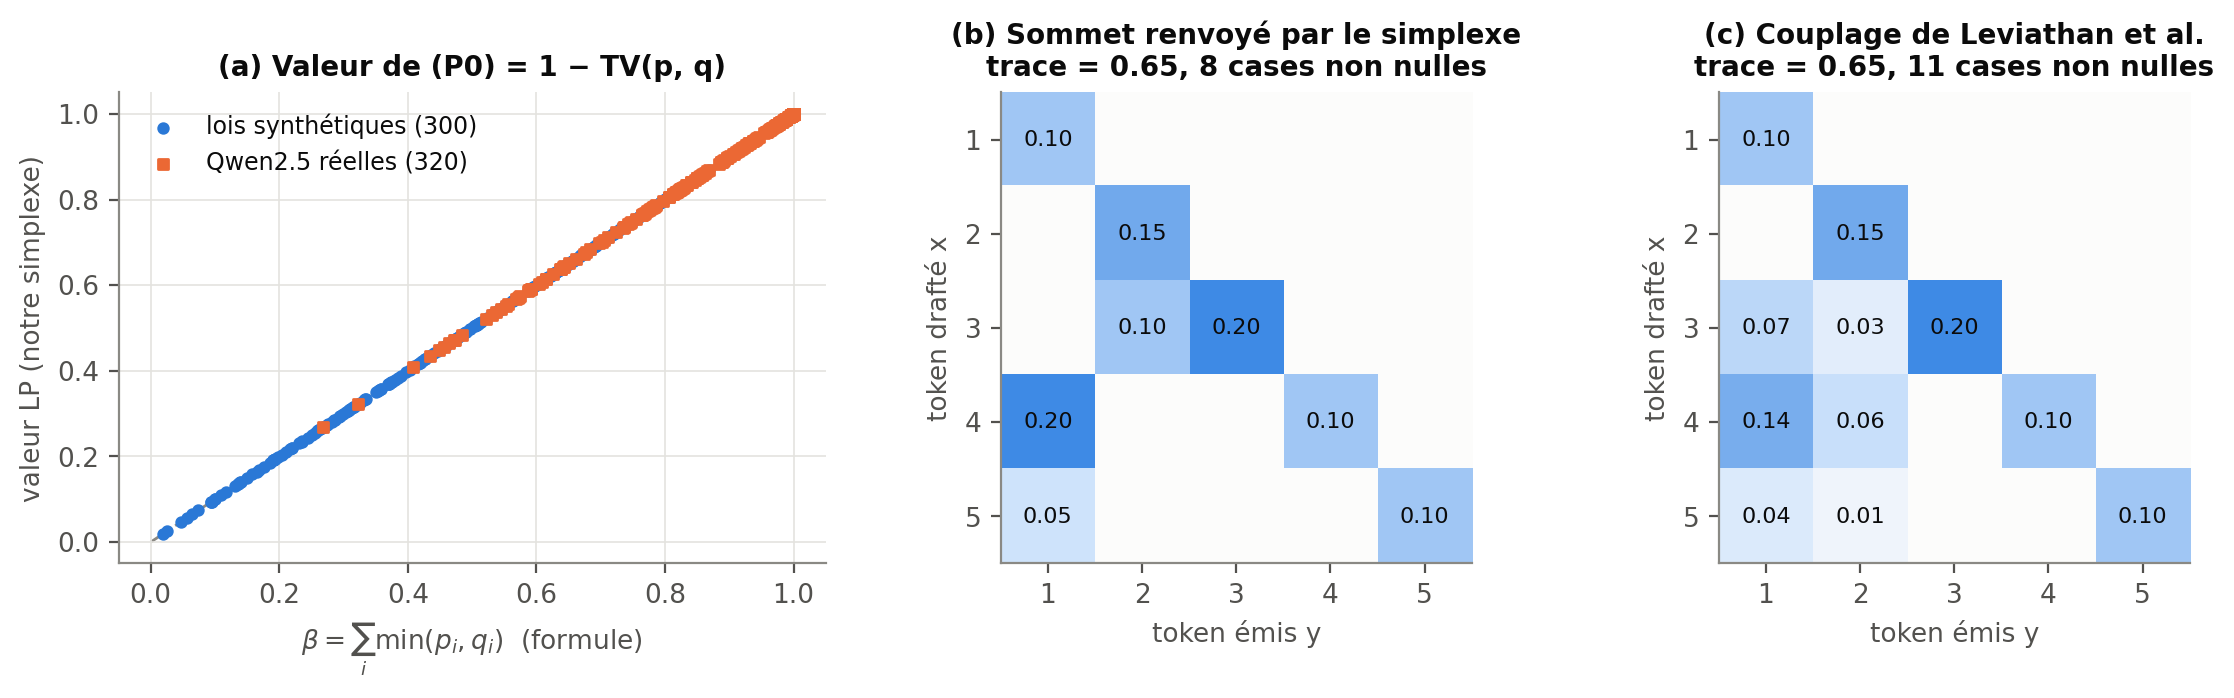
\includegraphics[width=0.78\linewidth]{fig1_lp_exact.png}
\caption{(a) La valeur de $(P_0)$ calculée par notre simplexe coïncide avec $\beta=\sum\min(p,q)$. (b-c) Deux couplages optimaux pour $p=(0{,}35;0{,}25;0{,}2;0{,}1;0{,}1)$ et $q=(0{,}1;0{,}15;0{,}3;0{,}3;0{,}15)$ : le sommet renvoyé par le simplexe (8 cases non nulles, au plus $2n-1=9$) et $\pi^L$, qui n'est pas un sommet (11 cases). Même diagonale, donc même acceptation $0{,}65$.}
\label{fig:lp}
\end{figure}

\begin{proposition}[valeur de $(P_0)$]\label{prop:valeur}
La valeur optimale de $(P_0)$ vaut $\beta(p,q)=\sum_x\min(p_x,q_x)=1-\TV(p,q)$.
Les solutions optimales sont exactement les $\pi\ge0$ telles que $\pi_{xx}=\min(p_x,q_x)$ pour tout $x$ et dont la partie hors diagonale a pour marges $(q-p)_+$ (lignes) et $(p-q)_+$ (colonnes).
La solution est unique si et seulement si l'un de ces deux vecteurs a au plus une composante non nulle.
\end{proposition}

\paragraph{Deux identités utilisées partout.} Pour deux réels $a,b$ : $\min(a,b)+(a-b)_+=a$ (cas $a\le b$ et $a>b$). Pour deux lois $p,q$, $\sum_x(p_x-q_x)_+=\sum_x(q_x-p_x)_+=\TV(p,q)$, car la différence de ces deux sommes vaut $\sum_x(p_x-q_x)=0$ et leur somme $\sum_x|p_x-q_x|=2\,\TV$. On en déduit $\beta=\sum_x\big(p_x-(p_x-q_x)_+\big)=1-\TV$.

\begin{proof}
\emph{Étape 1 : majoration.} Pour tout $\pi$ admissible, une case diagonale est inférieure à la somme de sa ligne et à celle de sa colonne (les autres cases sont $\ge0$) : $\pi_{xx}\le q_x$ et $\pi_{xx}\le p_x$, donc $\sum_x\pi_{xx}\le\beta$.

\emph{Étape 2 : la borne est atteinte par le couplage de Leviathan.} Si $\TV=0$, alors $p=q$ et $\diag(p)$ convient. Sinon, la règle de~\cite{leviathan} accepte $x$ avec probabilité $\min(1,p_x/q_x)$, et sinon tire $y$ selon $(p-q)_+/\TV$ ; elle induit le couplage
\[\pi^L=\underbrace{\diag\big(\min(p,q)\big)}_{\text{proposer }x\text{ et l'accepter}}+\underbrace{\frac{(q-p)_+\,(p-q)_+^{\top}}{\TV}}_{\text{proposer }x,\text{ rejeter, émettre }y}.\]
\begin{itemize}
\item Diagonale : $\Prob(\text{proposer }x\text{ et accepter})=q_x\min(1,p_x/q_x)=\min(p_x,q_x)$.
\item Hors diagonale : $\Prob(\text{proposer }x\text{ et rejeter})=q_x-\min(p_x,q_x)=(q_x-p_x)_+$, puis $y$ est tiré avec probabilité $(p_y-q_y)_+/\TV$.
\item Lignes : $\sum_y\pi^L_{xy}=\min(p_x,q_x)+(q_x-p_x)_+\,\frac{\sum_y(p_y-q_y)_+}{\TV}=\min(p_x,q_x)+(q_x-p_x)_+=q_x$.
\item Colonnes : $\sum_x\pi^L_{xy}=\min(p_y,q_y)+\frac{\sum_x(q_x-p_x)_+}{\TV}\,(p_y-q_y)_+=p_y$.
\item Trace : le terme de rang 1 est nul sur la diagonale, car $(q_x-p_x)_+(p_x-q_x)_+=0$. Donc $\sum_x\pi^L_{xx}=\beta$.
\end{itemize}
$\pi^L$ est admissible et atteint la borne de l'étape 1 : il est optimal, et la valeur de $(P_0)$ est $\beta$.

\emph{Étape 3 : forme de toutes les solutions.} Si $\pi$ est optimal, $\sum_x\pi_{xx}=\beta$ alors que $\pi_{xx}\le\min(p_x,q_x)$ pour tout $x$ : toutes ces inégalités sont des égalités. Il reste sur la ligne $x$ la masse $(q_x-p_x)_+$ et sur la colonne $y$ la masse $(p_y-q_y)_+$, à répartir hors diagonale (figure~\ref{fig:structure}). Une case $\pi_{xy}>0$ hors diagonale exige $q_x>p_x$ et $p_y>q_y$ ; ces deux ensembles étant disjoints, on a bien $x\ne y$. Réciproquement, tout $\pi\ge0$ de cette forme a les bonnes marges et la trace $\beta$.

\emph{Étape 4 : (non-)unicité.} Supposons que $\{q>p\}$ et $\{p>q\}$ contiennent chacun au moins deux tokens. Il existe alors $x\ne x'$ dans $\{q>p\}$ et $y\ne y'$ dans $\{p>q\}$ avec $\pi_{xy}>0$ et $\pi_{x'y'}>0$. En effet, chaque colonne $y\in\{p>q\}$ reçoit une masse $>0$, donc il existe $\pi_{x_1y_1}>0$ et $\pi_{x_2y_2}>0$ avec $y_1\ne y_2$ ; si $x_1\ne x_2$, c'est terminé ; sinon on prend une autre ligne $x'\in\{q>p\}$, qui a une case $\pi_{x'y''}>0$ avec $y''$ différent de $y_1$ ou de $y_2$, et l'on associe ces deux cases.
On remplace alors $\pi_{xy},\pi_{x'y'}$ par $\pi_{xy}-\delta,\pi_{x'y'}-\delta$ et $\pi_{xy'},\pi_{x'y}$ par $\pi_{xy'}+\delta,\pi_{x'y}+\delta$, avec $0<\delta\le\min(\pi_{xy},\pi_{x'y'})$ : chaque ligne et chaque colonne gagne et perd $\delta$, la diagonale est inchangée (les quatre cases sont hors diagonale, car $\{q>p\}$ et $\{p>q\}$ sont disjoints), et l'on obtient une autre solution optimale.
Si l'un des deux supports a au plus un élément, la partie hors diagonale est forcée (toute la masse va vers, ou vient de, ce seul token, ou il n'y a rien à placer) : la solution est unique.
\end{proof}

\begin{figure}[htbp]
\centering
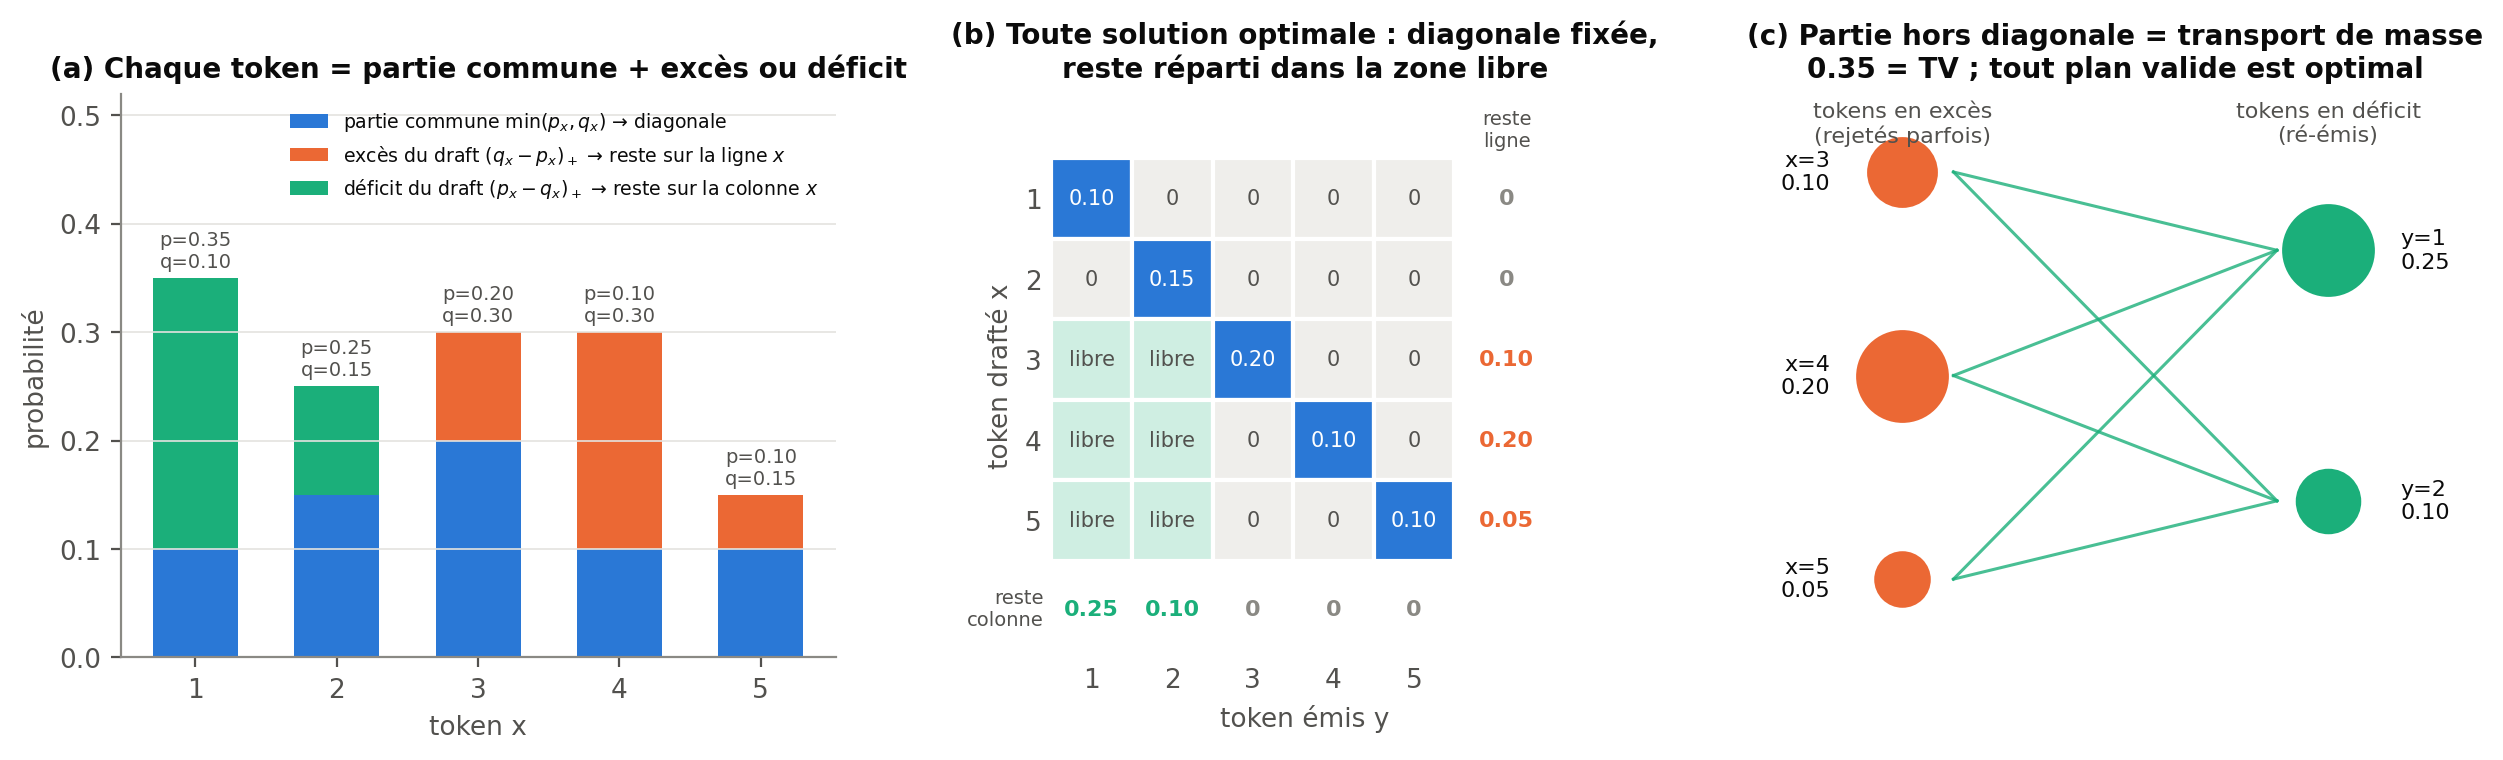
\includegraphics[width=0.78\linewidth]{fig1b_structure.png}
\caption{\emph{Étape 3 de la preuve}, sur l'exemple de la figure~\ref{fig:lp} : $p=(0{,}35;0{,}25;0{,}2;0{,}1;0{,}1)$, $q=(0{,}1;0{,}15;0{,}3;0{,}3;0{,}15)$.
(a) Chaque token se décompose en une partie commune $\min(p_x,q_x)$ (bleu), qui va sur la diagonale de $\pi$, plus soit un excès du draft $(q_x-p_x)_+$ (orange), soit un déficit $(p_x-q_x)_+$ (vert).
(b) Structure imposée à toute solution optimale : diagonale fixée à $\min(p,q)$ ; il reste $(q-p)_+$ à placer sur chaque ligne et $(p-q)_+$ sur chaque colonne. Une case hors diagonale ne peut être non nulle que si sa ligne a un reste et sa colonne un besoin (cases « libres » : lignes 3 à 5, colonnes 1 et 2).
(c) Remplir la zone libre revient à transporter la masse $\TV=0{,}35$ des tokens en excès vers ceux en déficit : tout plan de transport donne $\beta=0{,}65$.}
\label{fig:structure}
\end{figure}



\subsection{Dualité : un certificat d'optimalité explicite}\label{sec:dualite}
\paragraph{Écriture du dual.} D'après le cours, le dual de $\min\{c\cdot x:Ax=b,\ x\ge0\}$ est $\max\{b\cdot\mu:A^\top\mu\le c\}$. On note $\mu=(\varphi,\psi)\in\R^n\times\R^n$, où $\varphi_x$ est le multiplicateur de la contrainte « ligne $x$ » et $\psi_y$ celui de « colonne $y$ ». La colonne de $A$ associée à $\pi_{xy}$ contient un 1 sur la ligne $x$ et un 1 sur la ligne $n+y$, donc $(A^\top\mu)_{xy}=\varphi_x+\psi_y$ ; de plus $c_{xy}=-\delta_{xy}$ et $b\cdot\mu=q\cdot\varphi+p\cdot\psi$. D'où
\[(D_0)\qquad \max_{\varphi,\psi}\ q\cdot\varphi+p\cdot\psi\quad\text{s.c.}\quad \varphi_x+\psi_y\le-\delta_{xy}\quad\forall x,y.\]

\paragraph{Dualité faible, en une ligne.} Pour $\pi$ admissible et $\mu$ dual admissible, $c-A^\top\mu\ge0$ et $\pi\ge0$, donc
\[c\cdot\pi\ \ge\ (A^\top\mu)\cdot\pi=\mu\cdot(A\pi)=\mu\cdot b,\qquad\text{soit}\qquad -\sum_x\pi_{xx}\ \ge\ q\cdot\varphi+p\cdot\psi.\]
Si l'on exhibe $\pi$ et $\mu$ pour lesquels il y a égalité, les deux sont optimaux.

\paragraph{Le certificat.} Posons $S=\{x:q_x\le p_x\}$ (tokens que le draft ne sur-propose pas) et
\[\varphi_x=\begin{cases}-1&x\in S\\0&x\notin S\end{cases}\qquad \psi_y=\begin{cases}0&y\in S\\-1&y\notin S.\end{cases}\]
Sur la diagonale, exactement l'un des deux vaut $-1$, donc $\varphi_x+\psi_x=-1=c_{xx}$ ; hors diagonale, $\varphi_x+\psi_y\in\{0,-1,-2\}$, donc $\le0=c_{xy}$ : $(\varphi,\psi)$ est admissible. Sa valeur est $q\cdot\varphi+p\cdot\psi=-\sum_{x\in S}q_x-\sum_{y\notin S}p_y=-\sum_x\min(p_x,q_x)=-\beta$.
La valeur duale $-\beta$ égale la valeur primale $c\cdot\pi^L$ : par dualité faible, $\pi^L$ et $(\varphi,\psi)$ sont optimaux. On retrouve la proposition~\ref{prop:valeur} sans l'étape 1.

\paragraph{Écarts complémentaires.} À l'optimum, $\pi_{xy}>0\Rightarrow\varphi_x+\psi_y=c_{xy}$. Sur $\pi^L$ : une case hors diagonale non nulle a $q_x>p_x$ ($\varphi_x=0$) et $p_y>q_y$ ($\psi_y=0$), donc $\varphi_x+\psi_y=0=c_{xy}$ ; sur la diagonale, $\varphi_x+\psi_x=-1=c_{xx}$. \emph{Lecture :} $\varphi_x=-1$ marque les tokens que le draft propose « trop peu » ($q_x\le p_x$) : ils sont toujours acceptés.

\begin{suite}
$S=\{\tok{canapé},\tok{lit}\}$, donc $\varphi=(-1,-1,0)$ et $\psi=(0,0,-1)$ ; valeur duale $-(0{,}2+0{,}3)-0{,}2=-0{,}7=-\beta$, égale à la trace de $\pi^L$ (§\ref{sec:modeleI}). Seul \tok{tapis}, que le draft propose trop souvent, n'est pas toujours accepté : c'est le seul token de multiplicateur de ligne nul.
\end{suite}

\subsection{Algorithme : simplexe révisé en deux phases}\label{sec:simplexe}
Le simplexe est programmé comme dans le cours. Avec la base $\cB$ et les hors-base $\cN$ : $x_\cB=A_\cB^{-1}b$, multiplicateurs $\mu=A_\cB^{-\top}c_\cB$, coûts réduits $\tilde c_\cN=c_\cN-A_\cN^\top\mu$ ; si $\tilde c_\cN\ge0$, la base est optimale (critère d'optimalité du simplexe) ; sinon, la variable de coût réduit le plus négatif entre, et le test du ratio $\theta^*=\min\{x_{\cB,i}/d_i:d_i>0\}$, avec $d=A_\cB^{-1}A_j$, désigne la variable sortante. La phase~1 (variables artificielles) fournit une base admissible, ou prouve que le problème ne l'est pas. Les bases sont très dégénérées ($2n-1$ variables de base, souvent nulles) : pour exclure le cyclage, on passe à la règle de Bland après $2m$ pivots dégénérés consécutifs ($m=2n-1$ contraintes). Les multiplicateurs de la base finale donnent le dual (§\ref{sec:perte}).

\subsection{Validation numérique}\label{sec:validation}
Pour chaque $n=3,\dots,12$, on tire 30 paires $(p,q)$ selon des lois de Dirichlet plus ou moins piquées, des lois presque certaines (un LLM sûr de son prochain token) aux lois presque uniformes, et l'on compare la valeur de $(P_0)$ donnée par \textbf{notre simplexe}, par \textbf{HiGHS} (le solveur de référence de SciPy, développé indépendamment) et par la \textbf{formule} $\beta$. On prend aussi 320 positions réelles de GSM8K, en réduisant chaque paire de lois aux 6 tokens les plus probables de chaque modèle plus une case « autres » qui regroupe la masse restante.
\begin{center}
\small
\begin{tabularx}{\linewidth}{@{}lcX@{}}
\toprule
Comparaison & Écart maximal & Lecture\\\midrule
notre simplexe / formule $\beta$ & $4{,}4\times10^{-16}$ & précision machine (double précision)\\
HiGHS / formule $\beta$ & $4{,}4\times10^{-16}$ & idem\\
notre simplexe / formule, paires réelles & $3{,}5\times10^{-11}$ & masses minuscules (jusqu'à $10^{-12}$), sous la tolérance $10^{-10}$ du test d'optimalité\\
\bottomrule
\end{tabularx}
\end{center}
Le code est en Python ; 19 tests unitaires contrôlent notamment l'\textbf{admissibilité duale} $A^\top\mu\le c$, la \textbf{dualité forte} $b\cdot\mu=c\cdot x$, le certificat $(\varphi,\psi)$ du §\ref{sec:dualite} et la détection des problèmes non admissibles ou non bornés. Le nombre d'itérations croît environ comme $n^{1{,}7}$ (de 10 pour $n=3$ à 105 pour $n=12$) : pour un vrai vocabulaire ($n\approx150\,000$, plus de $2\times10^{10}$ variables), on calcule directement la formule fermée $\beta$, que le simplexe sert à \emph{vérifier}.

\paragraph{Ce que la validation a appris.} Elle ne remplace pas la preuve de la proposition~\ref{prop:valeur}, qui vaut pour toutes les lois, mais elle a révélé deux points : sans renormalisation, les lois réelles rendent $(P_0)$ non admissible (notre phase~1 le détecte) ; et un test qui attendait un prix dual égal à 1 en $\varepsilon=0$ a échoué, le simplexe renvoyant 2. Ce n'était pas une erreur, mais un coin de la fonction valeur, où tout prix $\ge1$ est valide (§\ref{sec:perte}).

\subsection{Vérification avec perte et prix dual du budget}\label{sec:perte}
\paragraph{Modèle.} On autorise la loi émise $r$ à s'écarter de $p$ d'au plus $\varepsilon$ en variation totale : la seconde marge de $\pi$ devient une variable $r$ ($r_y=\sum_x\pi_{xy}\ge0$ et $\sum_yr_y=\sum_xq_x=1$ : $r$ est automatiquement une loi), avec $\TV(r,p)\le\varepsilon$. La valeur absolue n'étant pas linéaire, on introduit $t_y\ge0$ avec $t_y\ge r_y-p_y$ et $t_y\ge p_y-r_y$, c'est-à-dire $t_y\ge|r_y-p_y|$. Alors $\sum_yt_y\le2\varepsilon$ implique $\TV(r,p)\le\varepsilon$ ; réciproquement, si $\TV(r,p)\le\varepsilon$, le choix $t_y=|r_y-p_y|$ est admissible. Les deux formulations ont donc les mêmes $(\pi,r)$ admissibles :
\[(P_\varepsilon)\qquad \max_{\pi,r,t\ge0}\ \sum_x\pi_{xx}\quad\text{s.c.}\quad
\begin{aligned}&\textstyle\sum_y\pi_{xy}=q_x,\qquad \sum_x\pi_{xy}=r_y,\\
&t_y\ge r_y-p_y,\quad t_y\ge p_y-r_y,\qquad \textstyle\sum_yt_y\le2\varepsilon.\end{aligned}\]
En forme standard, chaque inégalité reçoit une variable d'écart positive ; la dernière ligne a pour second membre $2\varepsilon$.

\begin{proposition}[frontière avec perte]\label{prop:perte}
La valeur de $(P_\varepsilon)$ vaut $\alpha^*(\varepsilon)=\min(1,\beta+\varepsilon)$. Elle est atteinte par $r_\varepsilon=p+\theta(q-p)$ avec $\theta=\min(1,\varepsilon/\TV(p,q))$ (et $\theta=1$ si $\TV=0$).
\end{proposition}

\begin{proof}
\emph{Majoration.} Pour $(\pi,r,t)$ admissible, $\pi$ est un couplage des lois $q$ et $r$ : la proposition~\ref{prop:valeur} appliquée à $(q,r)$ donne $\sum_x\pi_{xx}\le1-\TV(q,r)$. L'inégalité triangulaire $\TV(q,p)\le\TV(q,r)+\TV(r,p)$ donne alors
\[\sum_x\pi_{xx}\ \le\ 1-\TV(q,p)+\TV(r,p)\ \le\ \beta+\varepsilon,\]
et bien sûr $\sum_x\pi_{xx}\le\sum_{x,y}\pi_{xy}=1$.

\emph{Borne atteinte.} $r_\varepsilon$ est un mélange de $p$ et $q$, donc une loi ; $r_\varepsilon-p=\theta(q-p)$ donne $\TV(r_\varepsilon,p)=\theta\,\TV\le\varepsilon$, et $q-r_\varepsilon=(1-\theta)(q-p)$ donne $\TV(q,r_\varepsilon)=(1-\theta)\TV$. Le couplage de Leviathan entre $q$ et $r_\varepsilon$ accepte avec probabilité
\[1-(1-\theta)\TV=\beta+\theta\,\TV=\begin{cases}\beta+\varepsilon&\text{si }\varepsilon\le\TV\ (\theta=\varepsilon/\TV),\\1&\text{si }\varepsilon\ge\TV\ (\theta=1,\ r_\varepsilon=q).\end{cases}\qedhere\]
\end{proof}

\begin{suite}[$\varepsilon=0{,}1$]
$\theta=1/3$ et $r_\varepsilon=p+\tfrac13(q-p)=(0{,}4;0{,}3;0{,}3)$ : on émet un peu plus souvent \tok{tapis} que ne le voudrait le target ; $\TV(r_\varepsilon,p)=\tfrac12(0{,}1+0+0{,}1)=0{,}1$ et $\beta(q,r_\varepsilon)=0{,}2+0{,}3+0{,}3=0{,}8=\beta+\varepsilon$.
\end{suite}

\paragraph{Le multiplicateur du budget est une pente.} Soit $V(\varepsilon)=-\alpha^*(\varepsilon)$ la valeur en minimisation. L'ensemble dual $D=\{\mu:A^\top\mu\le c\}$ ne dépend pas de $\varepsilon$ ; seul le second membre $b(\varepsilon)=b_0+2\varepsilon\,e_{\text{budget}}$ en dépend. Par dualité forte, $V(\varepsilon)=\max_{\mu\in D}b(\varepsilon)\cdot\mu$ est convexe et, pour un dual optimal $\mu^*$ en $\varepsilon$, $V(\varepsilon')\ge b(\varepsilon')\cdot\mu^*=V(\varepsilon)+2\mu^*_B(\varepsilon'-\varepsilon)$. Le \textbf{prix du budget} $\kappa=-2\mu^*_B\ge0$ ($\mu^*_B\le0$, car l'écart de la ligne de budget a un coût nul) est donc un sur-gradient de $\alpha^*$ : le gain d'acceptation par unité de déviation. Il vaut 1 pour $\varepsilon<\TV$ et 0 au-delà, ce que renvoie le simplexe (figure~\ref{fig:perte}b) ; aux coins, il n'est pas unique (tout $\kappa\in[0,1]$ en $\varepsilon=\TV$, tout $\kappa\ge1$ en $\varepsilon=0$). \textbf{Une unité de déviation achète exactement une unité d'acceptation} tant qu'il reste du désaccord : c'est la frontière linéaire de~\cite{yin}, retrouvée avec les outils du cours, et la brique de la partie II.

\begin{figure}[htbp]
\centering
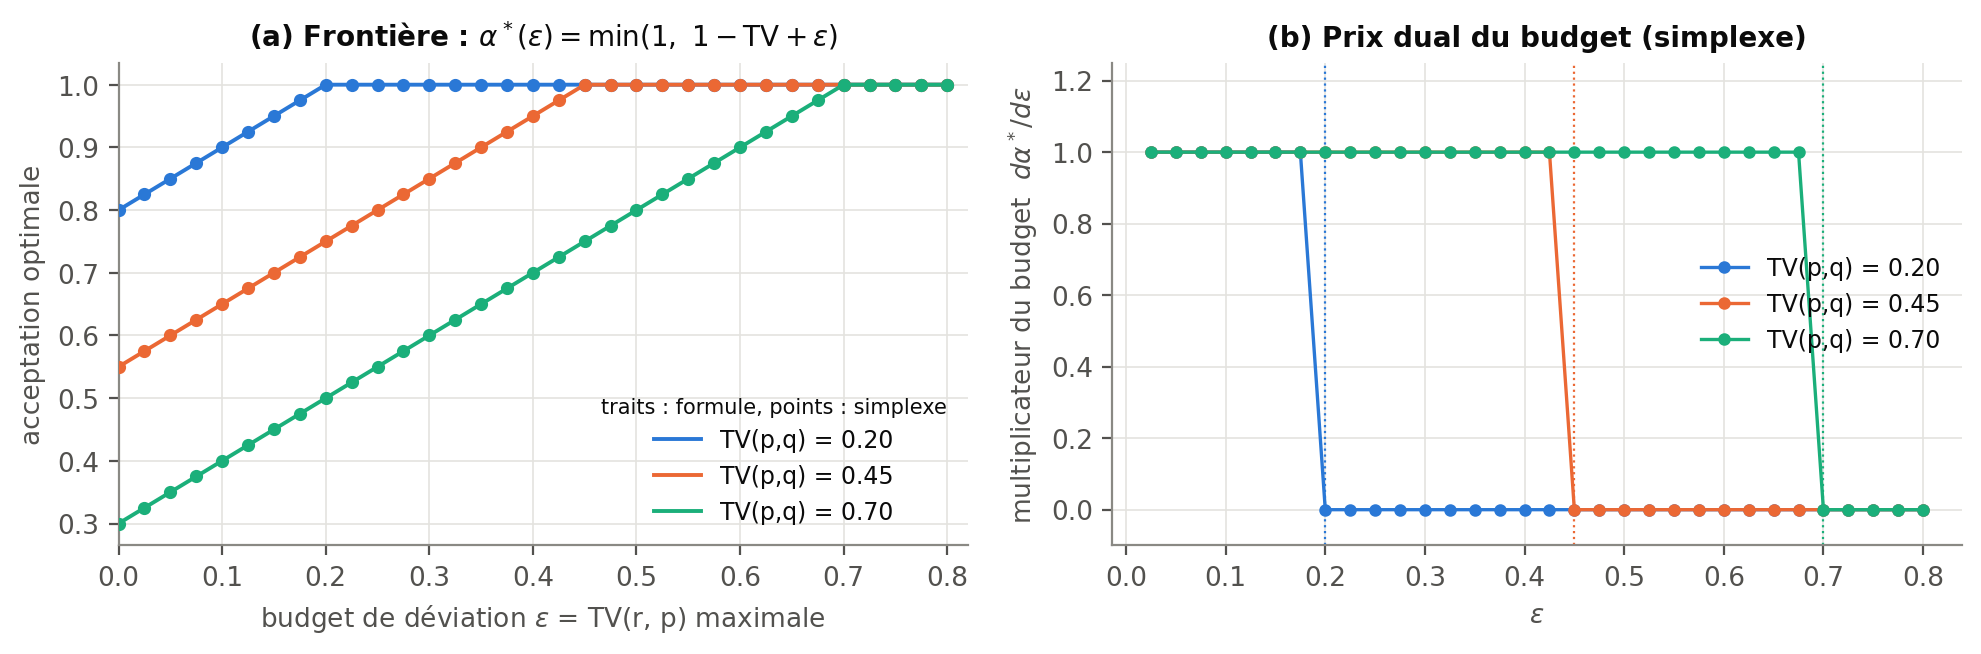
\includegraphics[width=0.74\linewidth]{fig2_lossy_frontier.png}
\caption{(a) Acceptation optimale en fonction du budget $\varepsilon$, pour trois paires $(p,q)$ ; points : simplexe, traits : proposition~\ref{prop:perte} (écart maximal $2{,}8\times10^{-16}$). (b) Prix du budget $\kappa=-2\mu^*_B=d\alpha^*/d\varepsilon$ calculé à partir du dual renvoyé par le simplexe : 1 avant $\varepsilon=\TV$ (pointillés), 0 après.}
\label{fig:perte}
\end{figure}

%=====================================================================
\section{Partie II : répartir le budget entre les positions d'un bloc}
%=====================================================================
\noindent\emph{En bref.} On dispose maintenant d'un budget de déviation pour tout un bloc. Dévier à la position $t$ augmente son acceptation (partie I) mais coûte $s_t$ par unité en qualité ; on cherche la répartition qui maximise le nombre moyen de tokens par passe du target, à budget de qualité donné (§\ref{sec:ou}).

\subsection{Modèle : variables, objectif, contraintes}\label{sec:modeleII}
Un bloc compte $\gamma$ positions draftées. La position $t$ a une acceptation exacte $a_t=\beta(p_t,q_t)\in(0,1)$ et une \textbf{sensibilité} $s_t>0$ : la baisse de qualité de la réponse finale par unité de déviation (en variation totale) à cette position.

\paragraph{Variables :} les déviations $\varepsilon=(\varepsilon_1,\dots,\varepsilon_\gamma)$. \textbf{Hypothèses :}
\begin{itemize}
\item[(H1)] les acceptations des différentes positions sont indépendantes, comme dans~\cite{leviathan} ;
\item[(H2)] la perte de qualité est additive au premier ordre : $\sum_ts_t\varepsilon_t$ ;
\item[(H3)] d'après la proposition~\ref{prop:perte}, relâcher la position $t$ de $\varepsilon_t$ donne l'acceptation $\alpha_t=a_t+\varepsilon_t$, avec $0\le\varepsilon_t\le u_t:=1-a_t=\TV_t$ (au-delà, l'acceptation vaut déjà 1). On appelle $u_t$ la \emph{marge} de la position $t$.
\end{itemize}

\paragraph{Objectif : nombre moyen de tokens par passe du target.} Soit $N$ le nombre de tokens draftés acceptés dans le bloc. Le bloc s'arrête au premier rejet, donc « au moins $k$ acceptés » signifie « les $k$ premiers acceptés » et, sous (H1),
\[\Prob(N\ge k)=\alpha_1\alpha_2\cdots\alpha_k=:P_k\qquad(P_0=1).\]
Pour une variable à valeurs entières, $\Esp[N]=\sum_{k\ge1}\Prob(N\ge k)$. Le target émet en plus un token à la fin de chaque passe (sa correction en cas de rejet, ou un token bonus si tout est accepté). D'où
\[E(\varepsilon)=1+\Esp[N]=1+\sum_{k=1}^{\gamma}\prod_{j=1}^{k}(a_j+\varepsilon_j).\]
C'est la formule de l'exemple du §\ref{sec:ou}, où le faible $a_2=0{,}5$ coupe la moitié des blocs.
\textbf{Contraintes :} $K=\{\varepsilon\in\R^\gamma:\ 0\le\varepsilon_t\le u_t,\ s\cdot\varepsilon\le B\}$, toutes affines.
\[(Q_B)\qquad \max_{\varepsilon\in K}\ E(\varepsilon)\qquad\Longleftrightarrow\qquad \min_{\varepsilon\in K}\ J(\varepsilon)=-E(\varepsilon).\]
\paragraph{Modèle de référence (modèle A).} Notre problème $(Q_B)$ est le \textbf{modèle B}, comme « bloc ». Pour mesurer ce que rapporte la prise en compte du bloc, on le compare à un modèle plus naïf, le \textbf{modèle A}, comme « additif ». Celui-ci fait comme si chaque position était vérifiée séparément, le rejet de l'une n'empêchant pas de vérifier les suivantes : le nombre moyen de tokens acceptés serait alors $\sum_t\alpha_t$, que le modèle A maximise sous les mêmes contraintes $K$. Comme $\sum_t\alpha_t=\sum_ta_t+\sum_t\varepsilon_t$, c'est le PL $\max_{\varepsilon\in K}\sum_t\varepsilon_t$, un sac à dos fractionnaire, qui relâche d'abord les positions les moins sensibles (§\ref{sec:kkt}) : c'est la règle que l'on appliquerait spontanément, « relâcher là où c'est le moins risqué ». Dans l'exemple du §\ref{sec:ou}, A voit le même gain ($+0{,}1$) à relâcher la position 2 ou la position 3, alors que le vrai gain vaut $0{,}162$ contre $0{,}045$ : il ignore que la position 3 n'est atteinte qu'une fois sur deux.


\subsection{Existence, structure et unicité}\label{sec:existenceII}
\paragraph{Existence.} $K$ est un polyèdre non vide ($0\in K$ car $B\ge0$), fermé et borné ($0\le\varepsilon\le u$), donc compact ; $J=-E$ est un polynôme, donc continu. Par le théorème de Weierstrass (une fonction continue sur un compact atteint son minimum), $J$ admet au moins un minimum, c'est-à-dire $E$ un maximum. C'est le théorème d'existence du cours, dont l'hypothèse de coercivité (« infinie à l'infini » : $\nr{\varepsilon_n}\to+\infty\Rightarrow J(\varepsilon_n)\to+\infty$ pour toute suite de $K$) est vraie par vacuité sur un ensemble borné, puisqu'aucune suite n'y tend vers l'infini.

\paragraph{Gradient.} $\alpha_t$ n'apparaît que dans les $P_k$ avec $k\ge t$, et linéairement : $\partial P_k/\partial\alpha_t=P_k/\alpha_t$ pour $k\ge t$, $0$ sinon. Comme $\partial\alpha_t/\partial\varepsilon_t=1$,
\[\partial_tE=\sum_{k\ge t}\frac{P_k}{\alpha_t}=P_{t-1}\big(1+\alpha_{t+1}+\alpha_{t+1}\alpha_{t+2}+\dots+\alpha_{t+1}\cdots\alpha_\gamma\big)=P_{t-1}\,T_t,\]
où $P_{t-1}$ est la \textbf{probabilité d'atteindre} la position $t$ et $T_t$ (défini par $T_\gamma=1$, $T_t=1+\alpha_{t+1}T_{t+1}$) le \textbf{nombre de tokens} que l'acceptation de $t$ « débloque », elle comprise. Tous les $\alpha_j$ sont $>0$, donc $\partial_tE>0$ : $E$ croît strictement en chaque variable.

\paragraph{Hessienne.} $E$ est affine en chaque $\alpha_t$ séparément (fonction multilinéaire), donc $\partial^2_{tt}E=0$. Pour $i<j$, $\alpha_j$ n'apparaît que dans $T_i$, et
\[\partial^2_{ij}E=P_{i-1}\Big(\prod_{i<k<j}\alpha_k\Big)T_j\ >0.\]

\paragraph{Non-concavité.} La hessienne $H$ est symétrique, non nulle et de trace nulle : ses valeurs propres sont réelles, de somme nulle et pas toutes nulles, donc l'une est $>0$. $H$ n'est semi-définie négative en aucun point : $E$ \textbf{n'est pas concave} ($J$ n'est pas convexe).

\begin{exemple}[$\gamma=2$, $a=(0{,}5;0{,}5)$]
$E=1+\alpha_1+\alpha_1\alpha_2$, $\nabla E=(1+\alpha_2,\alpha_1)$ et $H=\begin{psmallmatrix}0&1\\1&0\end{psmallmatrix}$, de valeurs propres $\pm1$. Sur la diagonale $\varepsilon_1=\varepsilon_2$ : $E(0;0)=1{,}75$, $E(0{,}5;0{,}5)=3$, mais $E(0{,}25;0{,}25)=2{,}3125$, \emph{sous} la corde $(1{,}75+3)/2=2{,}375$ ; une fonction concave serait au-dessus.
\end{exemple}

\paragraph{Lecture.} $\partial^2_{ij}E>0$ : relâcher une position augmente la valeur marginale des autres, qu'on atteint plus souvent (positions \textbf{complémentaires}). Les résultats d'unicité du cours, fondés sur la convexité stricte ou forte, ne s'appliquent pas, et l'on ne peut exclure a priori plusieurs maxima locaux.

\begin{lemme}[concavité le long des échanges]\label{lem:echange}
Pour deux positions $i\ne j$, la direction $d=s_je_i-s_ie_j$ conserve le coût ($s\cdot d=0$), et $h\mapsto E(\varepsilon+hd)$ est un trinôme strictement concave.
\end{lemme}
\begin{proof}
À coordonnées autres que $i,j$ fixées, $E$ est affine en $\alpha_i$ et en $\alpha_j$ séparément : $E=c_0+c_i\alpha_i+c_j\alpha_j+\partial^2_{ij}E\,\alpha_i\alpha_j$, où $\partial^2_{ij}E>0$ ne dépend ni de $\alpha_i$ ni de $\alpha_j$. Le long de $d$, $\alpha_i\leftarrow\alpha_i+hs_j$ et $\alpha_j\leftarrow\alpha_j-hs_i$ : le coefficient de $h^2$ vaut $-s_is_j\,\partial^2_{ij}E<0$.
\end{proof}
Transférer du budget d'une position à une autre est donc un problème concave en dimension~1 ; la non-concavité vient des directions qui font varier plusieurs positions dans le même sens, comme $\varepsilon_1=\varepsilon_2$ dans l'exemple. Ce lemme explique la proposition~\ref{prop:gamma2} et rend plausible l'unimodalité observée (§\ref{sec:algoII}).

\begin{lemme}[budget saturé]\label{lem:sature}
En tout maximum local, ou bien $s\cdot\varepsilon=B$, ou bien $\varepsilon=u$ (budget surabondant, $B\ge s\cdot u$).
\end{lemme}
\begin{proof}
Si $s\cdot\varepsilon<B$ et $\varepsilon_t<u_t$ pour un $t$, alors $\varepsilon+he_t\in K$ pour $h>0$ petit, et $E(\varepsilon+he_t)=E(\varepsilon)+h\,\partial_tE+o(h)>E(\varepsilon)$ puisque $\partial_tE>0$ : ce n'est pas un maximum local.
\end{proof}

\begin{proposition}[cas $\gamma=2$ : unicité et solution explicite]\label{prop:gamma2}
Si $B<s\cdot u$, le maximum est unique. On note $\kappa_s=s_1/s_2$ et $c=a_2+B/s_2$. Avec $\eta^*=\tfrac12\big((1+c)/\kappa_s-a_1\big)$, la solution est $\varepsilon_1^*=\mathrm{proj}_{[\eta_-,\eta_+]}(\eta^*)$ et $\varepsilon_2^*=(B-s_1\varepsilon_1^*)/s_2$, où $[\eta_-,\eta_+]=\big[\max\big(0,(B-s_2u_2)/s_1\big),\ \min\big(u_1,B/s_1\big)\big]$ est l'ensemble des $\varepsilon_1$ compatibles avec les bornes. Si $\eta_-<\eta^*<\eta_+$, la valeur optimale et le multiplicateur valent
\[E^*(B)=1+\frac{(1+c+\kappa_sa_1)^2}{4\kappa_s},\qquad \lambda^*=\frac{1+c+\kappa_sa_1}{2s_1}=\frac{dE^*}{dB}.\]
\end{proposition}
\begin{proof}
Par le lemme~\ref{lem:sature}, tout maximum est sur le segment $\{s\cdot\varepsilon=B\}\cap K$. On pose $\varepsilon_1=\eta$, $\varepsilon_2=(B-s_1\eta)/s_2$, soit $\alpha_1=a_1+\eta$ et $\alpha_2=c-\kappa_s\eta$ ; les bornes imposent $\eta\in[\eta_-,\eta_+]$. Alors
\[E(\eta)=1+(a_1+\eta)(1+c-\kappa_s\eta),\qquad E'(\eta)=(1+c)-\kappa_s(a_1+2\eta),\qquad E''(\eta)=-2\kappa_s<0.\]
$E$ est un trinôme strictement concave (c'est le lemme~\ref{lem:echange}) : son maximum sur un segment est unique, égal à $\eta^*$ (zéro de $E'$) projeté sur $[\eta_-,\eta_+]$. Si $\eta^*$ est intérieur, $a_1+\eta^*=(1+c+\kappa_sa_1)/(2\kappa_s)$ et $1+c-\kappa_s\eta^*=(1+c+\kappa_sa_1)/2$, d'où $E^*$. Enfin $c$ dépend de $B$ avec $dc/dB=1/s_2$, donc $dE^*/dB=(1+c+\kappa_sa_1)/(2\kappa_ss_2)=(1+\alpha_2^*)/s_1=\partial_1E/s_1=\lambda^*$ (§\ref{sec:kkt}).
\end{proof}
Dans ce régime, $E^*(B)$ est un polynôme de degré 2 en $B$, de coefficient dominant positif : la frontière est \emph{convexe} et le prix $\lambda^*$ croît avec $B$.


\begin{proposition}[positions identiques : relâcher d'abord le début]\label{prop:ordre}
Si $a_t\equiv a$ et $s_t\equiv s$, toute solution optimale vérifie $\alpha_1\ge\alpha_2\ge\dots\ge\alpha_\gamma$.
\end{proposition}
\begin{proof}
Supposons $\alpha_t<\alpha_{t+1}$ en un optimum et échangeons $\varepsilon_t$ et $\varepsilon_{t+1}$. Le point obtenu est admissible (mêmes marges, même coût). Pour $k<t$, $P_k$ ne contient ni $\alpha_t$ ni $\alpha_{t+1}$ ; pour $k\ge t+1$, il contient le produit $\alpha_t\alpha_{t+1}$, inchangé. Seul $P_t=P_{t-1}\alpha_t$ change et devient $P_{t-1}\alpha_{t+1}$ : $E$ augmente de $P_{t-1}(\alpha_{t+1}-\alpha_t)>0$, ce qui contredit l'optimalité.
\end{proof}

\begin{figure}[htbp]
\centering
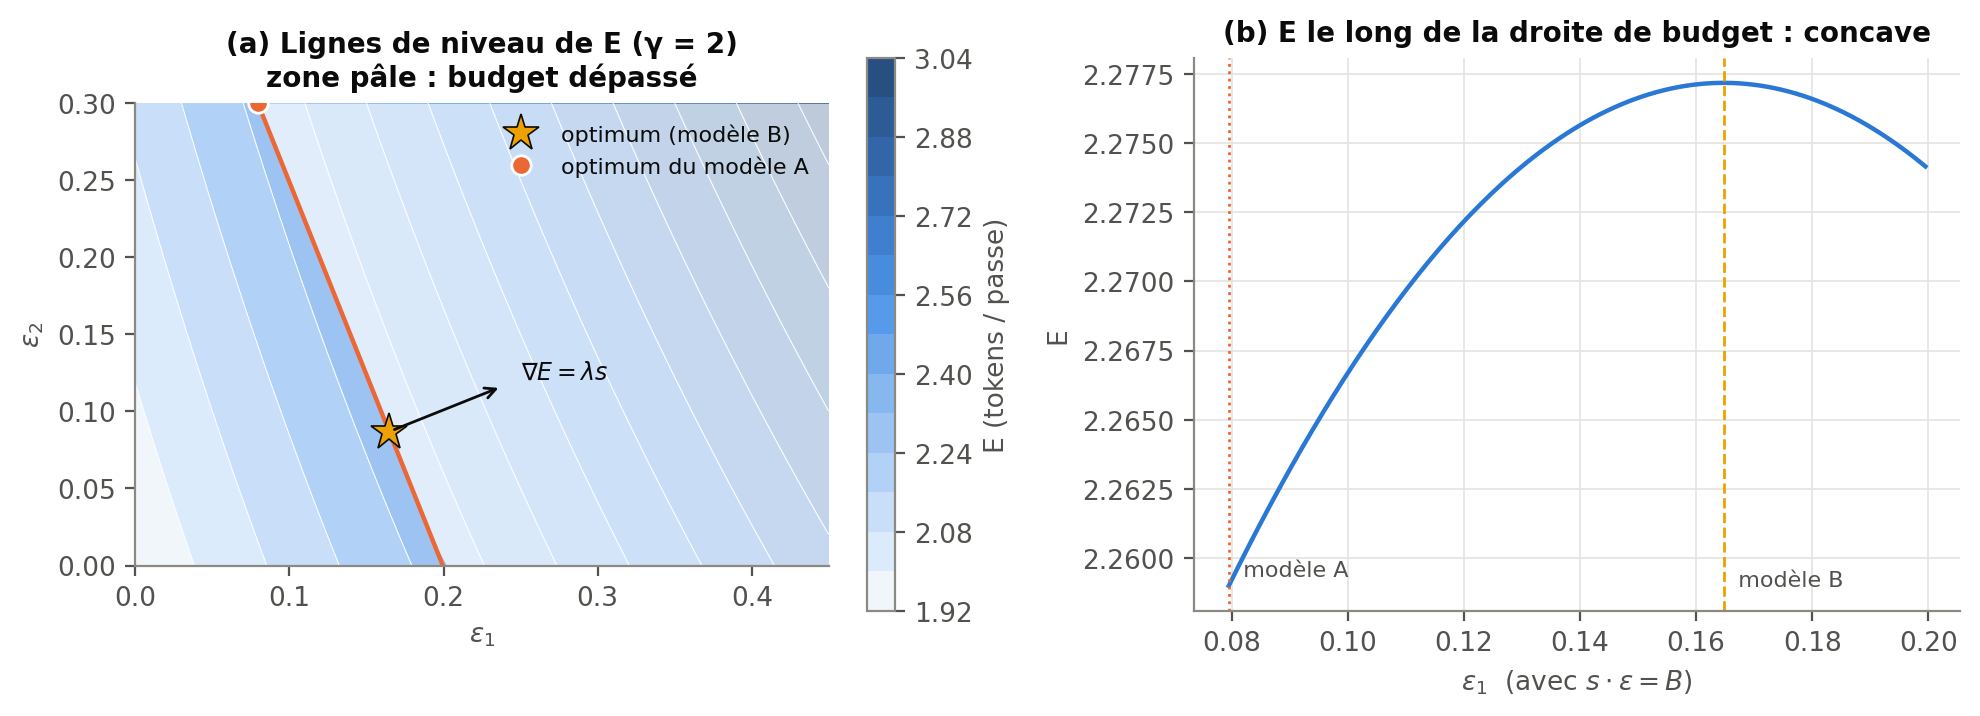
\includegraphics[width=0.72\linewidth]{fig3_landscape_gamma2.png}
\caption{$\gamma=2$, $a=(0{,}55;0{,}7)$, $s=(1{,}5;0{,}6)$, $B=0{,}35\,s\cdot u$. (a) À l'optimum $\varepsilon^*=(0{,}165;0{,}087)$, $\nabla E=\lambda s$ avec $\lambda=1{,}191=dE^*/dB$. (b) Le long de la droite de budget, $E$ est un trinôme concave ($E''=-5$) : $E^*=2{,}277$ (proposition~\ref{prop:gamma2}, retrouvé par le gradient projeté), contre $2{,}259$ pour le modèle A, qui choisit le bord.}
\label{fig:paysage}
\end{figure}

\subsection{Conditions d'optimalité (KKT)}\label{sec:kkt}
\paragraph{Contraintes.} On les écrit $F_i(\varepsilon)\le0$ : budget $s\cdot\varepsilon-B$ (gradient $s$, multiplicateur $\lambda\ge0$) ; bornes $-\varepsilon_t$ et $\varepsilon_t-u_t$ (gradients $-e_t$ et $e_t$, multiplicateurs $\mu^0_t,\mu^1_t\ge0$).

\paragraph{Qualification.} Toutes les $F_i$ sont affines. La qualification, au sens du cours, demande une direction $w$ telle que $\sca{\nabla F_i}{w}<0$ pour chaque contrainte active, l'égalité $\sca{\nabla F_i}{w}=0$ étant permise pour les contraintes affines : $w=0$ convient. On sait d'ailleurs que des contraintes affines sont toujours qualifiées : elles le sont en tout point de $K$.

\paragraph{Conditions KKT} (théorème de Karush-Kuhn-Tucker, appliqué à $J=-E$). En tout minimum local de $J$ (maximum local de $E$), il existe $\lambda,\mu^0,\mu^1\ge0$ tels que
\[\nabla J+\lambda s-\sum_t\mu^0_te_t+\sum_t\mu^1_te_t=0\quad\Longleftrightarrow\quad \nabla E(\varepsilon)=\lambda s-\mu^0+\mu^1,\]
avec les écarts complémentaires $\lambda(s\cdot\varepsilon-B)=0$, $\mu^0_t\varepsilon_t=0$ et $\mu^1_t(u_t-\varepsilon_t)=0$.
Ces conditions sont \textbf{seulement nécessaires} : $J$ n'est pas convexe, donc le théorème de Kuhn--Tucker, qui les rend suffisantes pour un problème convexe, ne s'applique pas. Un point KKT peut a priori être un maximum local non global, ou un point selle.

\paragraph{Lecture coordonnée par coordonnée.} Notons $\rho_t=\partial_tE/s_t$ le \textbf{rendement} de la position $t$ (tokens gagnés par unité de qualité perdue). La $t$-ième équation s'écrit $\partial_tE=\lambda s_t-\mu^0_t+\mu^1_t$ :
\begin{itemize}
\item si $0<\varepsilon_t<u_t$, aucune borne n'est active : $\mu^0_t=\mu^1_t=0$ et $\rho_t=\lambda$ ;
\item si $\varepsilon_t=0$ : $\mu^1_t=0$, donc $\rho_t\le\lambda$ (pas rentable, on ne relâche pas) ;
\item si $\varepsilon_t=u_t$ : $\mu^0_t=0$, donc $\rho_t\ge\lambda$ (très rentable, on relâche au maximum).
\end{itemize}
C'est une \textbf{règle de seuil} : on relâche les positions dont le rendement dépasse le prix $\lambda$. Pour le \textbf{modèle A}, $\rho_t=1/s_t$ ne dépend pas de $\varepsilon$, d'où le tri par sensibilité croissante (notre simplexe et cet algorithme glouton donnent la même solution). Pour le \textbf{modèle B}, $\rho_t=P_{t-1}T_t/s_t$ dépend de la \textbf{place} de la position : une position précoce est atteinte souvent ($P_{t-1}$ grand) et débloque beaucoup de tokens ($T_t$ grand). C'est pourquoi le budget va au début du bloc.

\paragraph{$\lambda$ est le prix marginal du budget.} Soit $\varepsilon^*$ optimal pour le budget $B$, avec une position intérieure $t$ ($0<\varepsilon^*_t<u_t$), et soit $0<h\le s_t\min(\varepsilon^*_t,u_t-\varepsilon^*_t)$. Le point $\varepsilon^*+(h/s_t)e_t$ est admissible pour le budget $B+h$, et $\varepsilon^*-(h/s_t)e_t$ pour le budget $B-h$. Comme $E$ est affine en $\varepsilon_t$ ($\partial^2_{tt}E=0$), $E$ y vaut exactement $E^*(B)\pm\partial_tE\,h/s_t=E^*(B)\pm\lambda h$. Donc $E^*(B+h)\ge E^*(B)+\lambda h$ et $E^*(B-h)\ge E^*(B)-\lambda h$, c'est-à-dire
\begin{equation}\label{eq:encadrement}
\frac{E^*(B)-E^*(B-h)}{h}\ \le\ \lambda\ \le\ \frac{E^*(B+h)-E^*(B)}{h}.
\end{equation}
Là où $E^*$ est dérivable, $\lambda=dE^*/dB$. C'est l'interprétation des multiplicateurs comme prix marginaux, vue en cours sous hypothèse de convexité ; ici, la structure multilinéaire de $E$ suffit. On le retrouve pour $\gamma=2$ (proposition~\ref{prop:gamma2}) et numériquement en S2, à 0,5\,\% près (figure~\ref{fig:frontiere}c).

\subsection{Algorithme : gradient projeté, et question des maxima locaux}\label{sec:algoII}
$K$ est convexe et la projection sur $K$ se calcule presque explicitement : on choisit le \textbf{gradient projeté} du cours, en montée,
\[\varepsilon_{k+1}=P_K\big(\varepsilon_k+\tau\nabla E(\varepsilon_k)\big).\]

\paragraph{1. Projection sur $K$.} $P_K(y)$ minimise $\tfrac12\nr{z-y}^2$, fortement convexe, sur le convexe fermé $K$ : d'après le cours, elle existe et est unique. En dualisant le budget avec $\nu\ge0$, le problème se sépare et donne $z_t(\nu)=\clip(y_t-\nu s_t,0,u_t)$. On prend $\nu=0$ si $s\cdot z(0)\le B$ ; sinon, $\Phi(\nu)=s\cdot z(\nu)$ décroît continûment de $\Phi(0)>B$ à $0$, et une dichotomie trouve $\Phi(\nu)=B$. Avec les multiplicateurs des bornes $\omega^0_t=(\nu s_t-y_t)_+$ et $\omega^1_t=(y_t-\nu s_t-u_t)_+$, $(z(\nu),\nu,\omega^0,\omega^1)$ vérifie KKT pour ce problème convexe à contraintes affines, où ces conditions sont suffisantes (théorème de Kuhn--Tucker) : $z(\nu)=P_K(y)$.

\paragraph{2. Choix du pas.} Sur $K$, $\alpha\in[0,1]^\gamma$ donne $|\partial^2_{ij}E|\le\gamma-\max(i,j)+1$ ; la norme de Frobenius majorant la norme de la hessienne, $\nabla E$ est $L$-lipschitzien sur $K$ avec
\[L=\Big(\sum_{i\ne j}\big(\gamma-\max(i,j)+1\big)^2\Big)^{1/2}.\]
Pour $\gamma=2$, $L=\sqrt2$ (la vraie norme de $H$ vaut 1) ; pour $\gamma=8$, $L\approx25{,}9$. On prend $\tau=1/L$.

\paragraph{3. Convergence.} Le théorème de convergence du gradient projeté vu en cours suppose $J$ fortement convexe : il \textbf{ne s'applique pas} ici, et pour la même raison ni les résultats sur l'algorithme d'Uzawa ni ceux sur la pénalisation. On démontre en annexe~\ref{app:convergence}, avec l'inéquation d'Euler, que $E(\varepsilon_k)$ croît, que les pas tendent vers 0 et que toute valeur d'adhérence de $(\varepsilon_k)$ vérifie les conditions KKT. Pour un problème non concave, c'est la meilleure garantie générale : un point KKT n'est pas forcément un maximum global.

\paragraph{4. Global ou local ?} On lance le gradient projeté depuis 20 points initiaux aléatoires sur 100 instances aléatoires ($\gamma\in\{3,4,6,8\}$ ; la hessienne y est indéfinie, comme en tout point d'après le §\ref{sec:existenceII}). L'écart maximal entre valeurs finales vaut $1{,}8\times10^{-15}$, l'écart maximal entre solutions $1{,}1\times10^{-8}$, et le résidu KKT maximal $2{,}9\times10^{-10}$. Nous n'avons donc \textbf{jamais observé deux maxima locaux distincts} : le problème est non concave mais, empiriquement, unimodal. L'unicité n'est démontrée que pour $\gamma=2$ (proposition~\ref{prop:gamma2}). Sur une instance $\gamma=8$, la convergence est linéaire : 279 itérations avec $\tau=1/L$, 62 avec $\tau=4/L$ (la montée n'est alors plus garantie, voir l'annexe~\ref{app:convergence}), et 40 départs aléatoires aboutissent à la même valeur $E^*=5{,}4544$.


\subsection{Résultats : où placer la déviation ?}\label{sec:resultats}
On prend $\gamma=6$, $a_t=0{,}6$ et un budget $B=0{,}3\,B_{\max}$ (où $B_{\max}=s\cdot u$), avec trois profils de sensibilité (figure~\ref{fig:allocation}).
\begin{itemize}
\item \textbf{S1 (positions identiques, $s_t=1$).} Le modèle B relâche dans l'ordre $1,2,\dots$ (proposition~\ref{prop:ordre}). Le modèle A est \emph{indifférent} : tous les $\rho_t=1/s$ sont égaux, donc toute répartition de même coût est A-optimale, y compris « fin d'abord », qui ne donne que $E=2{,}54$ contre $4{,}12$.
\item \textbf{S2 (début plus sensible, $s=(2;1{,}7;1{,}4;1{,}1;0{,}8;0{,}5)$).} Le modèle A relâche les dernières positions, les moins chères. Le modèle B relâche malgré tout les \textbf{premières} : $E=3{,}52$ contre $2{,}79$ pour A ($+26\,\%$) et $3{,}21$ pour une déviation uniforme. À l'optimum, $\rho_1=\rho_2=\lambda=1{,}308$ (positions intérieures) et $\rho_t<\lambda$ ailleurs, comme le prévoit KKT.
\item \textbf{S3 (deux tokens pivots, $s=2{,}5$ en positions 2 et 5, $0{,}3$ ailleurs).} Le modèle B évite le pivot tardif (position 5) mais relâche en partie le pivot précoce (position 2), qui conditionne l'accès aux positions 3 et 4. L'écart avec A est faible ($4{,}98$ contre $4{,}96$).
\end{itemize}

\begin{figure}[htbp]
\centering
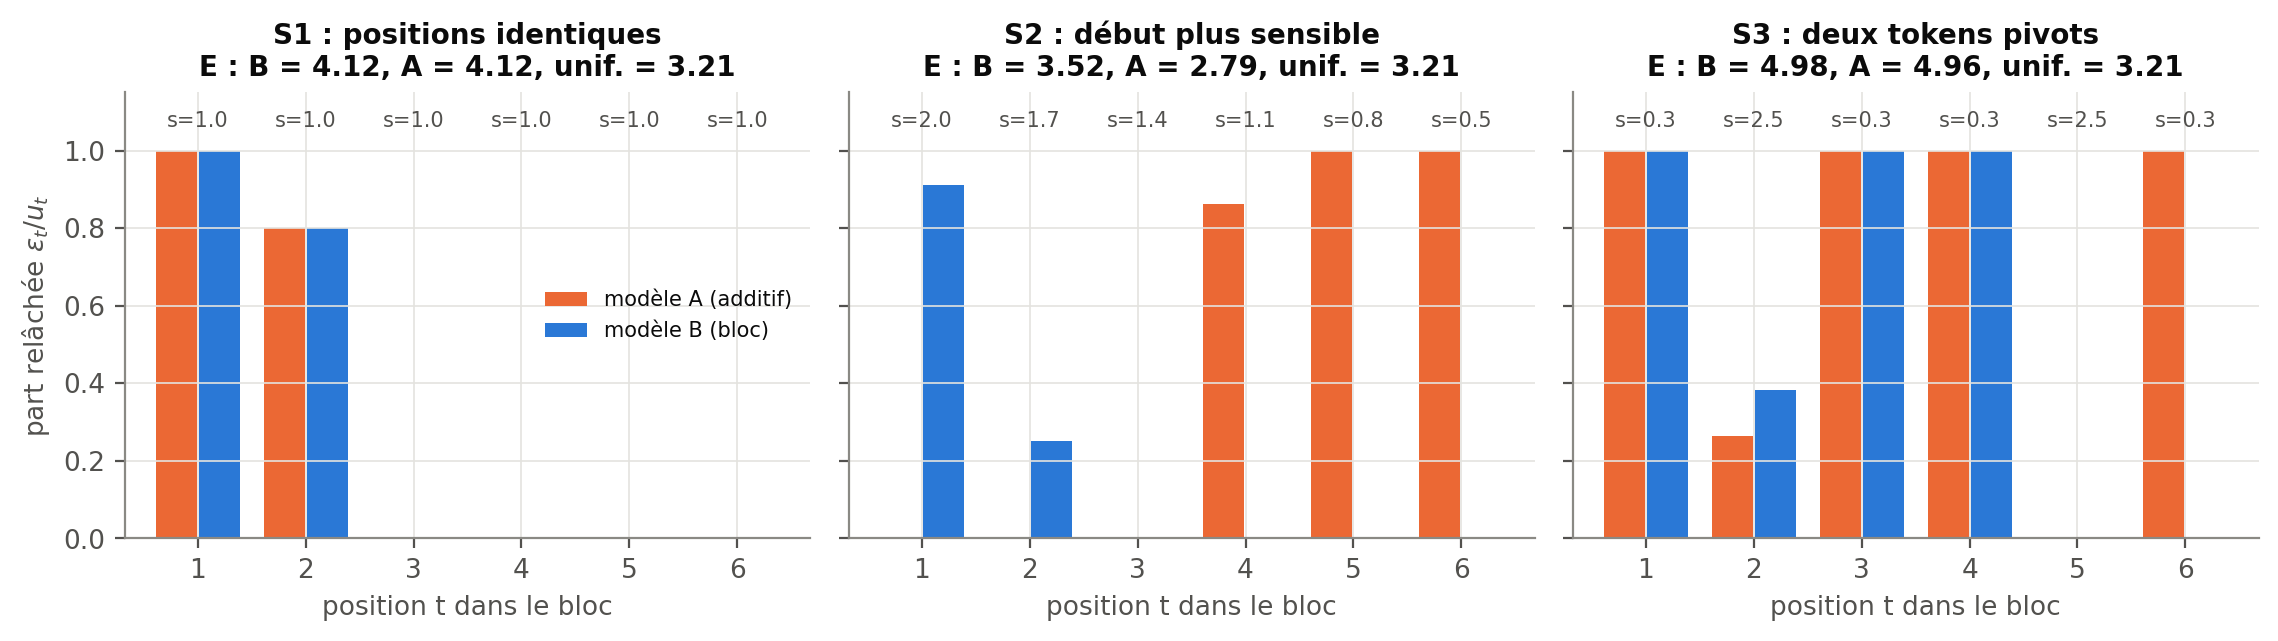
\includegraphics[width=0.8\linewidth]{fig5_allocation.png}
\caption{Part relâchée $\varepsilon_t/u_t$ par position, pour le modèle additif A (orange) et le modèle par blocs B (bleu). Les sensibilités $s_t$ sont indiquées au-dessus de chaque position.}
\label{fig:allocation}
\end{figure}

\paragraph{Frontière vitesse--budget (figure~\ref{fig:frontiere}).} Pour chaque budget, on compare l'optimum aux heuristiques. En S2, le gain maximal sur A vaut 0,97 token par passe, et sur la déviation uniforme 0,40. L'heuristique « fin d'abord » relâche le moins les premiers tokens, à la manière de~\cite{secure} qui vérifie plus strictement le début pour la sécurité ; du point de vue de la vitesse, elle est toujours la pire (à égalité avec A en S2).

La forme de la frontière $E^*(B)$ dépend du profil. En \textbf{S2}, elle est convexe et $\lambda^*(B)$ croît (figure~\ref{fig:frontiere}c) : l'effet de complémentarité des positions ($\partial^2_{ij}E>0$) domine, et il vaut mieux concentrer la déviation sur quelques positions que de la diluer (seules les deux premières sont relâchées, figure~\ref{fig:allocation}). En \textbf{S3}, au contraire, la frontière est essentiellement concave (figure~\ref{fig:frontiere}b) : sa pente décroît d'un segment à l'autre, car on dépense d'abord sur les positions bon marché ($s_t=0{,}3$), très rentables, puis sur les pivots, chers, comme dans un sac à dos. Les deux effets coexistent : en général, $E^*(B)$ n'est ni convexe ni concave.

L'encadrement~\eqref{eq:encadrement} dit où la pente peut baisser. Pour $B<s\cdot u$, le budget est saturé (lemme~\ref{lem:sature}). Si de plus $B$ n'est pas l'une des valeurs « sommets » $B_I=\sum_{t\in I}s_tu_t$ ($I\subset\{1,\dots,\gamma\}$), l'optimum n'est pas un sommet du pavé : il a une position intérieure, et \eqref{eq:encadrement} donne en $B$ une droite d'appui locale de pente $\lambda$, située sous $E^*$. Or une fonction continue qui admet une telle droite en tout point d'un intervalle est convexe sur cet intervalle\footnote{Si $f$ passait strictement au-dessus d'une de ses cordes sur $[c,d]$, la différence $g$ entre $f$ et la corde atteindrait un maximum $>0$ en un $x_0\in\,]c,d[$. La droite d'appui en $x_0$ a forcément la pente de la corde (sinon $g$ dépasserait $g(x_0)$ d'un côté de $x_0$), donc $g=g(x_0)$ près de $x_0$ : l'ensemble où $g$ atteint son maximum serait non vide, ouvert et fermé dans $[c,d]$, sans contenir $c$ ni $d$, ce qui contredit la connexité. $E^*$ est bien continue, et même localement lipschitzienne : si $\varepsilon'$ est optimal pour $B'>B>0$, le point $(B/B')\varepsilon'$ est admissible pour $B$.}. Ainsi, \textbf{$E^*$ est convexe entre deux valeurs $B_I$ consécutives, et sa pente ne peut baisser qu'en un $B_I$}. En S3, l'optimum relâche l'une après l'autre les positions bon marché 1, 3 et 4, puis le pivot précoce 2 (un temps avec la position 6), et le pivot tardif 5 en dernier : la pente chute en $B_I$ pour $I=\{1\}$, $\{1,3\}$, $\{1,3,4\}$ et $\{1,2,3,4,6\}$, d'où l'allure concave.

\begin{figure}[htbp]
\centering
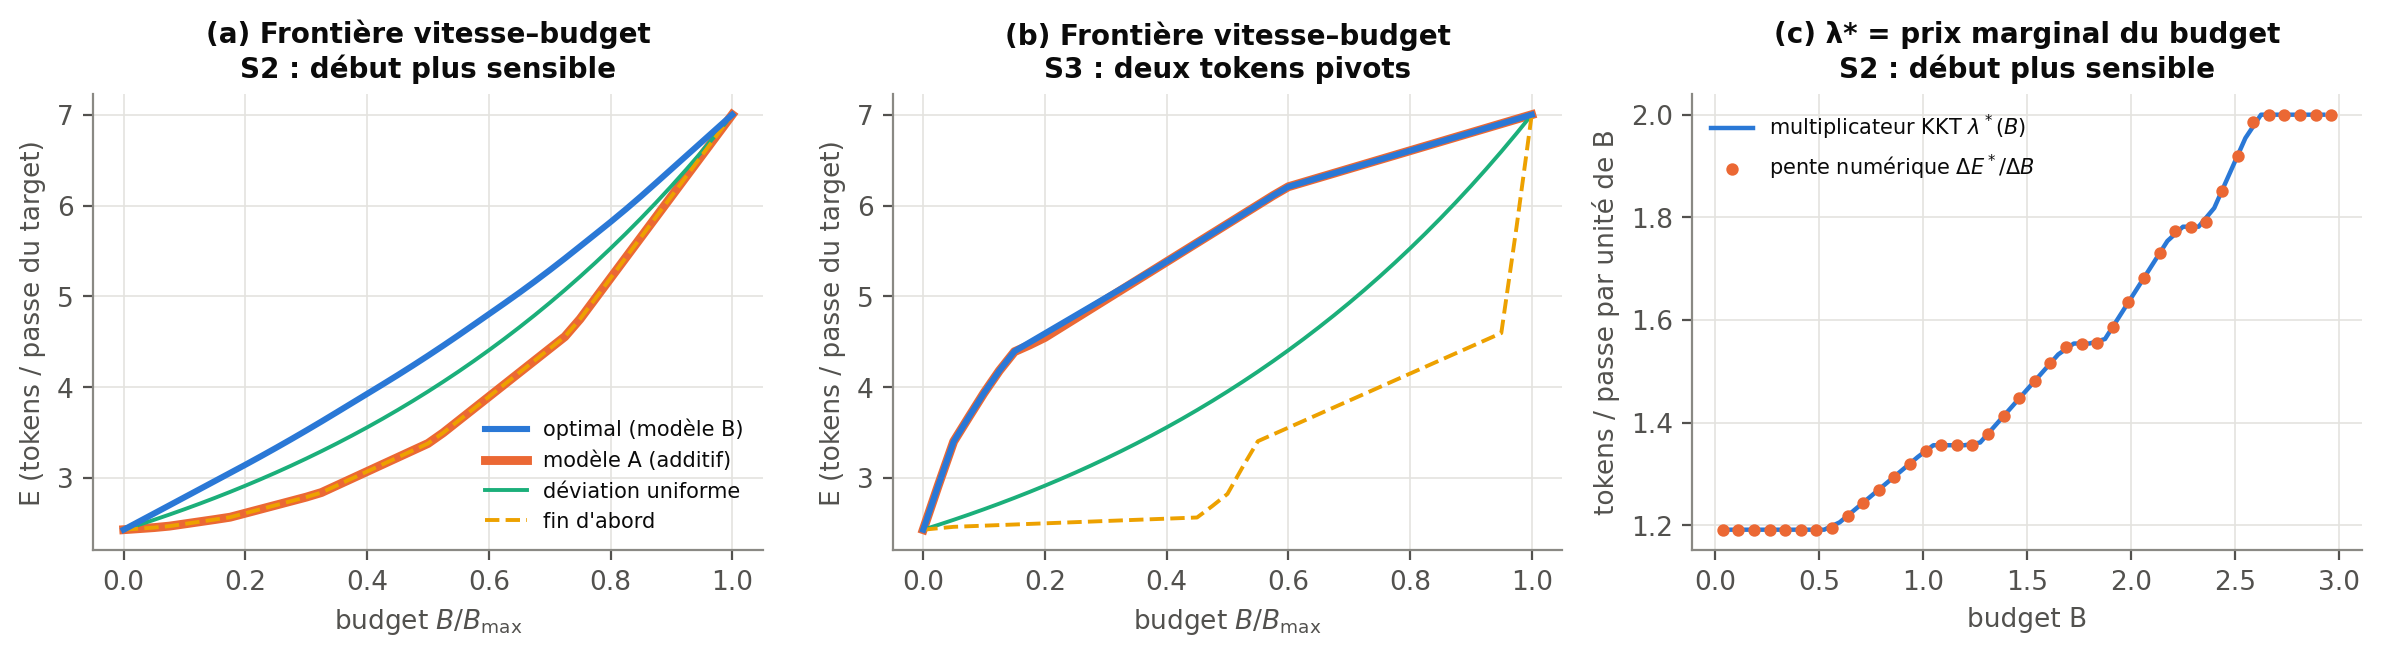
\includegraphics[width=0.72\linewidth]{fig6_frontier.png}
\caption{(a-b) Tokens par passe selon le budget, pour l'optimum et trois heuristiques. (c) En S2, $\lambda^*(B)$ coïncide avec la pente numérique $\Delta E^*/\Delta B$.}
\label{fig:frontiere}
\end{figure}

%=====================================================================
\section{Données réelles : Qwen2.5-1.5B (target) et Qwen2.5-0.5B (draft) sur GSM8K}\label{sec:reel}
%=====================================================================
Le target (Qwen2.5-1.5B) rédige des solutions à 16 problèmes GSM8K (2344 tokens) ; à chaque position, on calcule $a_t=\beta(p_t,q_t)$ sur le vocabulaire complet, avec le draft Qwen2.5-0.5B. L'acceptation exacte moyenne vaut 0,893, et 47\,\% des positions ont $a_t>0{,}99$ (figure~\ref{fig:reel}a) ; elle vaut 0,982 sur les tokens contenant un chiffre, souvent recopiés de l'énoncé. Les sensibilités n'étant pas mesurées dans ce DM, on prend le proxy $s_t=10$ pour les tokens contenant un chiffre et $s_t=1$ sinon, et l'on optimise des blocs de $\gamma=5$ sous un budget commun. À $B=0{,}2\,B_{\max}$, on obtient 5,18 tokens par passe (optimum), contre 4,98 (modèle A) et 4,87 (uniforme) ; le gain est plus faible qu'en synthétique, car la plupart des positions réelles ont déjà $a_t\approx1$ (figure~\ref{fig:reel}b). L'optimum relâche la première position du bloc à 73\,\% de sa marge, la deuxième à 43\,\% et les suivantes à 0\,\%, là où A répartit uniformément (22 à 28\,\%, figure~\ref{fig:reel}c) : on retrouve sur données réelles que la déviation doit aller au \textbf{début} du bloc.

\begin{figure}[htbp]
\centering
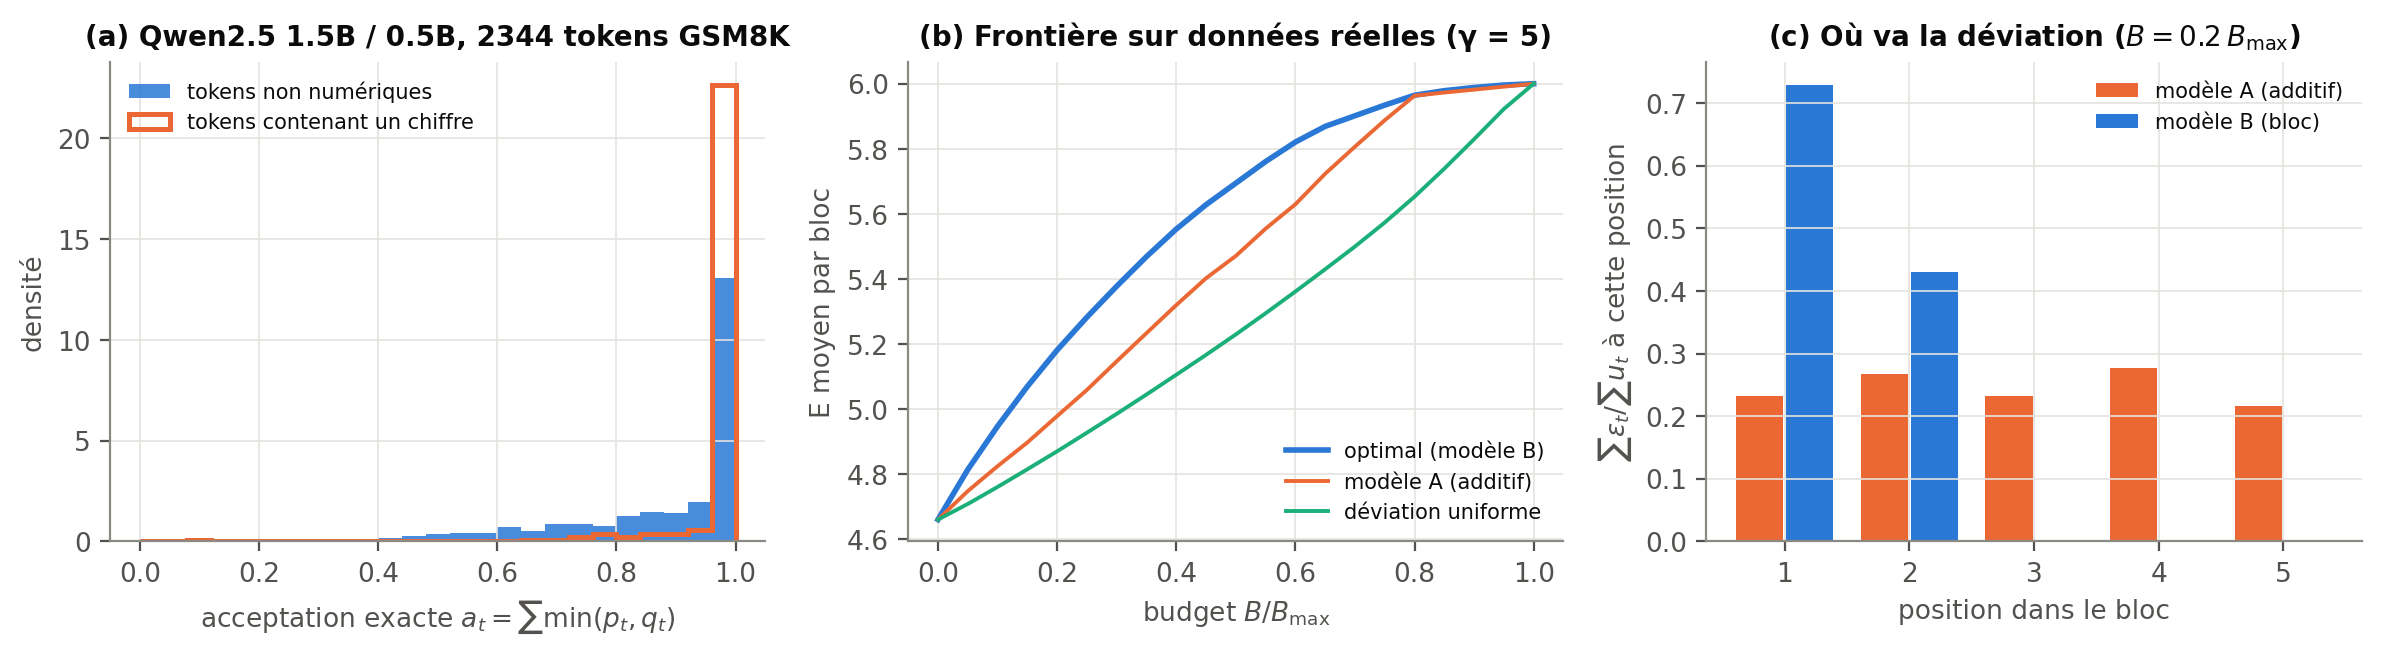
\includegraphics[width=0.66\linewidth]{fig7_real_data.png}
\caption{(a) Acceptations exactes mesurées. (b) Frontière vitesse--budget réelle. (c) Part relâchée par position, à $B=0{,}2\,B_{\max}$.}
\label{fig:reel}
\end{figure}

%=====================================================================
\section{Conclusion, limites et lien avec le projet}
%=====================================================================
Les deux problèmes se traitent avec les outils du cours : la partie I par le simplexe et la dualité (valeur $1-\TV$, certificat explicite, prix d'une unité de déviation) ; la partie II, non concave, par KKT (règle de seuil, dont le seuil $\lambda$ est le prix marginal exact du budget) et le gradient projeté, qui aboutit au même point KKT depuis tous nos départs.

Le message pour notre projet de recherche : \textbf{la structure en bloc change la réponse}. Une règle qui relâche les tokens peu sensibles sans tenir compte de leur position (modèle A) peut perdre plus d'un cinquième de la vitesse atteignable (en S2, 2,79 tokens par passe contre 3,52). Et la vitesse pousse à relâcher le début du bloc, à l'opposé des heuristiques de sécurité qui le vérifient plus strictement~\cite{secure} : cette tension est à quantifier avec de vraies sensibilités.

\textbf{Limites.} (H1) ignore la corrélation entre positions, (H2) est une approximation au premier ordre, les blocs réels se recalent après chaque rejet, et nos sensibilités sont des hypothèses que le projet devra mesurer.

%=====================================================================
\appendix
\section{Convergence du gradient projeté (cas non concave)}\label{app:convergence}
%=====================================================================
Notons $g=\nabla E(\varepsilon_k)$, $\varepsilon^+=\varepsilon_{k+1}=P_K(\varepsilon_k+\tau g)$, $d=\varepsilon^+-\varepsilon_k$, et $0<\tau<2/L$.
\begin{enumerate}
\item \textbf{Projection.} $P_K(y)$ minimise la fonction convexe $\tfrac12\nr{z-y}^2$ sur le convexe $K$ ; l'inéquation d'Euler, nécessaire et ici suffisante, donne
\begin{equation*}\label{eq:A1}
z^*=P_K(y)\iff z^*\in K\ \text{ et }\ \sca{z^*-y}{w-z^*}\ge0\quad\forall w\in K.\tag{A.1}
\end{equation*}
Avec $y=\varepsilon_k+\tau g$, $z^*=\varepsilon^+$ et $w=\varepsilon_k$ : $\sca{d-\tau g}{-d}\ge0$, soit $\sca{g}{d}\ge\nr{d}^2/\tau$.
\item \textbf{Montée.} Sur le segment $[\varepsilon_k,\varepsilon^+]\subset K$, $\nabla E$ est $L$-lipschitzien ; par Taylor avec reste intégral, $E(\varepsilon^+)\ge E(\varepsilon_k)+\sca{g}{d}-\frac L2\nr{d}^2$, d'où
\begin{equation*}\label{eq:A3}
E(\varepsilon_{k+1})\ \ge\ E(\varepsilon_k)+\Big(\frac1\tau-\frac L2\Big)\nr{\varepsilon_{k+1}-\varepsilon_k}^2,\qquad \frac1\tau-\frac L2>0.\tag{A.2}
\end{equation*}
\item \textbf{Conséquences.} $E(\varepsilon_k)$ croît et reste majorée par $1+\gamma$, donc en sommant \eqref{eq:A3}, $\nr{\varepsilon_{k+1}-\varepsilon_k}\to0$. $K$ étant compact, une sous-suite $\varepsilon_{k_j}$ converge vers $\bar\varepsilon$, ainsi que $\varepsilon_{k_j+1}$ ; par continuité de $P_K$ et de $\nabla E$, $\bar\varepsilon=P_K\big(\bar\varepsilon+\tau\nabla E(\bar\varepsilon)\big)$.
\item \textbf{Point fixe $\iff$ Euler $\iff$ KKT.} Par \eqref{eq:A1}, ce point fixe équivaut à $\sca{\nabla E(\bar\varepsilon)}{w-\bar\varepsilon}\le0$ pour tout $w\in K$ : la condition nécessaire d'Euler pour un minimum local de $J=-E$ sur $K$, équivalente aux conditions KKT du §\ref{sec:kkt} puisque les contraintes sont affines (lemme de Farkas).
\end{enumerate}
Rien ne garantit que $\bar\varepsilon$ soit le maximum \emph{global} : d'où les multi-départs.

\begin{thebibliography}{9}\footnotesize\setlength{\itemsep}{0pt}\setlength{\parskip}{0pt}
\bibitem{leviathan} Y.~Leviathan, M.~Kalman, Y.~Matias. \emph{Fast Inference from Transformers via Speculative Decoding}. ICML 2023.
\bibitem{chen} C.~Chen et al. \emph{Accelerating Large Language Model Decoding with Speculative Sampling}. {\NoAutoSpacing arXiv:2302.01318}, 2023.
\bibitem{yin} M.~Yin, M.~Chen, K.~Huang, M.~Wang. \emph{A Theoretical Perspective for Speculative Decoding Algorithm}. NeurIPS 2024.
\bibitem{fuzzy} M.~Holsman, Y.~Huang, B.~Dhingra. \emph{Fuzzy Speculative Decoding for a Tunable Accuracy-Runtime Tradeoff}. Findings of ACL 2025.
\bibitem{secure} Y.~Zhang, Z.~Wang, N.~Gong, Y.~Yang. \emph{Secure Speculative Decoding for Large Language Models}. {\NoAutoSpacing arXiv:2610.08678}, 2026.
\bibitem{allaire} G.~Allaire. \emph{Analyse numérique et optimisation}. Éditions de l'École polytechnique.
\end{thebibliography}
\end{document}
